% =========================================================================
% main.tex — Overleaf-ready LaTeX port of the UvA MSc thesis manuscript.
%
% COMPILE-UNVERIFIED: this scaffold was hand-converted from the canonical
% Markdown manuscript (thesis/*.md) on a machine with no TeX toolchain.
% It has NOT been compiled. Expect minor fixups on the first Overleaf
% compile. See thesis/latex/README.md for import instructions.
%
% Source of truth: thesis/00-abstract.md … thesis/09-appendix-provenance.md
% (wording is governed by chaosprobe/docs/explanation/scope-of-claims.md;
% no content changes were made in this port).
% =========================================================================
\documentclass[11pt,a4paper]{report}

\usepackage[utf8]{inputenc}
\usepackage[T1]{fontenc}
\usepackage{lmodern}
\usepackage[a4paper,margin=2.5cm]{geometry}
\usepackage{graphicx}
\usepackage{booktabs}
\usepackage{natbib}
\usepackage[hidelinks]{hyperref}

\bibliographystyle{plainnat}

% Figures live in thesis/figures/ (one level above this directory);
% the Overleaf project must contain both thesis/latex/ and thesis/figures/.
\graphicspath{{../figures/}}

% ----- Author-owned placeholders (TODO: fill in before submission) -----
\newcommand{\thesistitle}{Measuring the Impact of Chaos in Differing Placement Strategies within Cloud Systems}
\newcommand{\thesisauthor}{Yvo Hu}
\newcommand{\thesisdegree}{MSc Thesis, University of Amsterdam}
\newcommand{\thesissupervisor}{TODO: supervisor name}
\newcommand{\thesisexaminer}{TODO: second reader / examiner}
\newcommand{\thesisdate}{TODO: defense date}
\newcommand{\thesisprogramme}{TODO: programme name (e.g.\ Master Software Engineering)}

\begin{document}

% ----------------------------- Title page -------------------------------
\begin{titlepage}
  \centering
  {\scshape\large University of Amsterdam\par}
  {\large \thesisprogramme\par}
  \vspace{3cm}
  {\huge\bfseries \thesistitle\par}
  \vspace{1.5cm}
  {\Large \thesisauthor\par}
  \vspace{0.5cm}
  {\large \thesisdegree\par}
  \vfill
  \begin{tabular}{ll}
    Supervisor: & \thesissupervisor \\
    Examiner:   & \thesisexaminer   \\
  \end{tabular}
  \vspace{1cm}
  {\par\large \thesisdate\par}
\end{titlepage}

% ------------------------------ Abstract --------------------------------
\begin{abstract}
Kubernetes offers multiple placement mechanisms and rich observability, yet
it remains unclear when pod placement materially affects resilience under
chaos, and when aggregate resilience scores obscure that effect. This thesis
presents \textbf{ChaosProbe}, a Kubernetes chaos-evaluation framework that varies
pod-placement strategies, injects LitmusChaos faults into the Online Boutique
microservice benchmark, and stores provenance-stamped experiment
data. Measurement is layered: every outcome is read simultaneously at the
aggregate-score, kernel/network-mechanism, and user-visible layers. Using
ChaosProbe, we conduct a bounded empirical study across three fault classes ---
churn, load contention, and node failure. The primary evidence is a
seven-session campaign of independent, provenance-gated runs, plus
replicated load and node-drain batches.

The central finding is a measured latency$\leftrightarrow$availability trade-off: the same
co-location that minimizes inter-service latency under load maximizes blast
radius under node failure --- and a single aggregate score sees none of it.
Beneath that trade-off sits a layered decoupling that recurs across fault
classes: placement reproducibly moves mechanism-layer signals that do not
reproducibly reach the user. Under churn, spreading the target's dependents
flushes far more kernel conntrack state than co-locating them, in 7 of 7
independent sessions --- yet no stable user-visible advantage follows. The
aggregate score cannot rank placement strategies under session variance
(ICC 0.033). Under load, co-located services keep calls node-local and
hold 1.36--1.39$\times$ lower inter-service tail latency than spread across two
replicated batches; the user-visible effect did not survive replication and
is not claimed. A graph-derived cross-node fraction separates node-local from
spreading placements before any chaos is injected, and that separation
replicates; a continuous correlation did not and is not claimed. Under node
failure, draining the node hosting the target took 11 of 11 services offline
under colocate versus 2 of 11 under spread, and observed blast equaled
placement-predicted blast for every strategy.

These results show that placement under chaos should not be evaluated with a
single score alone: resilience conclusions depend on both the fault class and
the measurement layer. The thesis contributes a reproducible experimental
framework, a bounded empirical study whose every quoted number traces to an
archived run, and practical guidance for evaluating placement-sensitive
resilience claims in Kubernetes.
\end{abstract}

\tableofcontents

% ------------------------------ Chapters --------------------------------
% Ported from thesis/01-introduction.md — wording unchanged.
\chapter{Introduction}\label{ch:intro}

\section{Problem}\label{sec:problem}

The placement literature says \textbf{where pods land matters}: locality lowers
inter-service latency (NetMARKS, TraDE), interference makes co-location risky
(Bubble-Up, Quasar), and schedulers from Borg to Medea encode spread- and
packing-heuristics precisely because topology is assumed to drive performance
and availability. Chaos-engineering practice, meanwhile, evaluates resilience
by injecting faults and \textbf{collapsing the outcome into an aggregate score} ---
a single number per experiment (cf.\ the CSUR multi-vocal review: outcomes are
defined solely against steady-state user-visible indicators).

These two bodies of practice have not been connected: nobody has measured \emph{at
which layer} a placement effect appears under a given fault class, and whether
an aggregate score can see it at all. If placement moves a kernel-level
mechanism but not the user-visible outcome --- or moves availability but not
latency --- a single score is the wrong instrument, and placement advice derived
from it is unreliable.

Consider the concrete decision this thesis instruments. An operator runs a
ten-service microservice storefront on a small Kubernetes cluster and must
choose how to place it: pack the services onto as few nodes as possible, or
spread them across all of them. The packing intuition comes from the
network-aware scheduling literature --- co-located services keep their calls
node-local, and schedulers built on that observation report response-time
reductions of up to 37\% \citep{wojciechowski2021netmarks}.
The spreading intuition comes from the availability literature --- replicas and
services in distinct failure domains survive the loss of any one of them
\citep{garefalakis2018medea} ---
and from the interference literature, which warns that co-location invites
resource contention \citep{mars2011bubbleup,delimitrou2014quasar}.

What does today's tooling tell this operator? The Kubernetes scheduler scores
nodes on resource fit, not fault isolation --- a design it inherits from Borg
\citep{verma2015borg,burns2016borg} --- so the default
placement answers a different question than the one the operator is asking.
Chaos-engineering tools answer the resilience question directly, but they
answer it with one number: inject a fault, probe the steady state, emit a
score. Whether that score can actually \emph{discriminate} between the packed and
the spread placement --- whether its between-strategy signal exceeds its
run-to-run noise --- is, to our knowledge, unexamined.

The cost of choosing wrong is real on both axes, and asymmetric. If the
operator spreads when latency was the binding constraint, every inter-service
call crosses the network and the tail latency budget erodes continuously,
under exactly the load conditions where it matters most. If the operator packs
when availability was the binding constraint, the failure of a single node
takes the whole application down at once --- a blast-radius failure mode the
cloud-architecture literature warns about qualitatively
\citep{aws-cellbased}
but that placement-evaluation tooling does not measure. And if the operator
trusts an aggregate resilience score to adjudicate, they may be reading noise:
this thesis measures the score's reliability for exactly this ranking task and
finds it insufficient in the regime studied (H1, \S\ref{sec:h1}).

This thesis connects the two bodies of practice. We build a framework that
\emph{manipulates} placement as a controlled variable, injects faults from three
distinct classes, and measures the outcome at three layers simultaneously ---
the aggregate score, the kernel/network mechanism, and the user-visible
routes --- so that the question ``does placement matter under chaos?'' can be
answered per fault class and per layer rather than with a single number.

\section{Research question}\label{sec:rq}

% Verbatim from chaosprobe/docs/explanation/hypotheses.md — do not reword.

\begin{quote}
\textbf{Under which chaos fault classes does pod placement measurably affect
mechanism-level behaviour and user-visible outcomes in a Kubernetes
microservice application, and when do aggregate resilience scores obscure
those effects?}
\end{quote}

This is framed as a \textbf{fault-class-by-measurement-layer} study, not a
placement ranking and not a refutation of the placement literature. A
placement effect can appear at (a) the aggregate-score layer, (b) a
kernel/network mechanism layer, and/or (c) the user-visible layer, and these
layers need not agree --- so the contribution is establishing \emph{at which layer}
an effect appears under a given fault class, and whether it reaches the user.

We decompose the main question into four sub-questions, one per fault class
and one for the instrument itself:

\begin{itemize}
\item \textbf{SQ1 (churn).} Under single-replica \texttt{pod-delete} churn, at which
  measurement layer does a placement effect appear, and does it propagate to
  the user-visible routes? (Answered by H2 and H3, \S\ref{sec:h2}--\ref{sec:h3}.)
\item \textbf{SQ2 (load contention).} Under sustained load --- the regime where the
  user-visible outcome \emph{is} latency --- does placement move the inter-service
  mechanism, and does that effect reach the user-facing routes reproducibly?
  (Answered by H4 and H5, \S\ref{sec:h4}--\ref{sec:h5}.)
\item \textbf{SQ3 (node failure).} Under a node drain, how does placement move the
  availability axis --- blast radius and recovery time --- and how does that
  relate to the latency axis measured under load? (Answered by H6, \S\ref{sec:h6}.)
\item \textbf{SQ4 (score reliability).} Can the aggregate resilience score rank
  placement strategies at all, given session-level variance, at any feasible
  iteration count? (Answered by H1, \S\ref{sec:h1}.)
\end{itemize}

In crosswalk form: SQ1 $\rightarrow$ H2/H3, SQ2 $\rightarrow$ H4/H5, SQ3 $\rightarrow$ H6, SQ4 $\rightarrow$ H1.

SQ4 is logically prior to the others: if the standard instrument could rank
placements reliably, the layered measurement design would be a refinement.
Because it cannot (in this regime), the layered design is what produces the
findings at all.

The study that answers these questions, at a glance: eight placement
strategies (a no-fault control, the default scheduler, and six controlled
mutations spanning packing, spreading, randomization, and graph-aware
placement), realized by deployment-level \texttt{nodeSelector} mutation on the
Online Boutique benchmark --- ten polyglot gRPC microservices plus Redis, one
replica per service --- on a pinned five-node cluster (Kubernetes v1.28.6,
kube-proxy in ipvs mode). The churn evidence is a seven-session campaign of
independent, provenance-gated run invocations (8 strategies $\times$ 3 iterations
per session, 147 iterations); the load-contention evidence is two replicated
four-iteration batches under a 200-user spike; the node-failure evidence is
two clean node-drain batches. Every quoted number traces to an archived run
(Appendix~\ref{app:provenance}), and the single-replica scoping --- which makes \texttt{pod-delete} a
pure churn fault and excludes multi-replica failover questions --- is carried
explicitly through every claim (Chapter~\ref{ch:threats}).

\section{Contributions}\label{sec:contributions}

The thesis makes four explicit claims. The claims are ordered by decreasing
novelty; claim 1 itself bundles three findings of differing novelty, stated
separately so each is a one-line falsifiable target:

\begin{enumerate}
\item \textbf{Novel empirical contribution} --- three findings:
  \begin{itemize}
  \item \textbf{1a --- layered decoupling.} Under both single-replica churn and load
    contention, placement reproducibly moves a mechanism-layer signal
    (conntrack flush 38.5\% vs 2.7\%, H2; east-west tail 1.36--1.39$\times$, H4) that
    does \textbf{not} reproducibly reach the user-visible layer (H3, H4).
  \item \textbf{1b --- measured trade-off pair.} The same co-location property that
    minimizes east-west tail latency (H5) maximizes node-failure blast
    radius and recovery time (11/11 vs 2/11 services offline; $\approx$10.3 s vs
    $\approx$2.6 s, H6).
  \item \textbf{1c --- score-reliability critique.} The aggregate resilience score
    cannot rank placement strategies under session variance (ICC 0.033;
    between-strategy variance 3.3\% of total, H1).
  \end{itemize}

\item \textbf{Engineering contribution.} \textbf{ChaosProbe}: a placement-aware
  chaos-evaluation framework --- a placement mutator with eight strategies, a
  LitmusChaos experiment runner, cross-layer probers (Prometheus mechanism
  metrics, route latency, Redis, disk, resources, EndpointSlice snapshots),
  Locust load generation, and a Neo4j dependency/topology graph that H5 makes
  \textbf{analytically load-bearing} (the cross-node fraction is computed from the
  graph, not merely stored in it).

\item \textbf{Replication/validation contribution.} A \emph{provenance-gated multi-session
  campaign protocol}: independent single-commit sessions as the unit of
  analysis, every session gated by \texttt{doctor --strict} (scenario hashes,
  kube-proxy mode, environment fingerprint), every quoted number traceable to
  an archived run (Appendix~\ref{app:provenance}).

\item \textbf{Pilot/appendix contribution.} Documented negative findings --- CPU/memory
  hog faults absorbed by cgroup limits (scores $\approx$ 100), the \texttt{node-memory-hog}
  self-eviction autopsy --- and the discussion-tier H7 thread (target-scoped
  cross-node fraction as a flush predictor).
\end{enumerate}

\textbf{What the candidate did versus what the tooling did.} Because the
framework automates heavily, we state the division of labor plainly.
\emph{Authored for this thesis}: the placement mutator and all eight strategies;
the three-layer measurement design with its dependent-vs-control route
confound check; the cross-node-fraction metric (H5) and the blast-radius
trough measurement (H6); the provenance gate (\texttt{doctor --strict}), the
discard-not-patch rule, and the multi-session campaign protocol; the
churn-vs-contention fault-class framing; every committed analysis script
(variance partition, paired tests, TOST, figure generation); and the
judgment calls the gate forced --- including retracting two of our own
headline numbers (\S\ref{sec:retractions}). \emph{Integrated off-the-shelf}: LitmusChaos (fault
execution), Prometheus/Locust (collection and load), Neo4j (graph storage),
and the Online Boutique application. The science --- what to vary, what to
measure, what to believe --- is the candidate's; the third-party components
execute it.

Claim 1 is substantiated by Chapters \ref{ch:results} and \ref{ch:discussion}. Chapter~\ref{ch:results} reports each
hypothesis with its data, statistics, and archived provenance; Chapter~\ref{ch:discussion}
argues that the three results are one structure --- placement effects are real
but layer-bound, the two faces of co-location are the same graph property
read on opposing axes, and the aggregate score sees none of it. Every part of
the claim is bounded by Chapter~\ref{ch:threats}: it is a statement about single-replica
deployments on one small virtualized cluster, with the \emph{direction} of the
mechanism effects and the \emph{method} as the portable parts, not the absolute
numbers.

Claim 2 is substantiated by Chapter~\ref{ch:chaosprobe}, which describes the framework against
its actual code layout and documents the design decisions that the empirical
chapters depend on: deployment-level placement mutation with per-iteration
match-rate verification, cross-layer probing with explicit metric-availability
bookkeeping, and provenance stamping of every run. The framework is open and
the analysis scripts that produce each quoted number are committed alongside
it.

Claim 3 is substantiated by Chapter~\ref{ch:methodology} and Appendix~\ref{app:provenance}. The campaign protocol ---
independent run invocations, each on a single code commit, each gated by an
automated provenance and data-quality check before its numbers may be used ---
is what separates the headline results (7/7-session mechanism replication,
campaign-level variance decomposition) from the pilot tier. Appendix~\ref{app:provenance} maps
every claim to the archived runs that carry it.

Claim 4 is substantiated by Appendix~\ref{app:negative} and discussed in Chapters \ref{ch:methodology} and \ref{ch:discussion}. The
negative findings are presented as methodological results in their own right:
they explain \emph{why} the obvious contention experiments probe the wrong layer on
clusters of this class, and they redirect the experimental design toward load
as the contention stressor --- a lesson that future placement-under-chaos
studies can reuse directly.

\section{Thesis outline}\label{sec:outline}

Chapter~\ref{ch:related} positions the thesis against four bodies of literature --- resilience
profiling, production resilience testing, scheduler and placement research,
and measurement methodology --- and locates it at their empty intersection.
Chapter~\ref{ch:chaosprobe} describes ChaosProbe, the framework that produces all data in the
study, and its provenance-capture design. Chapter~\ref{ch:methodology} defines the three-layer
measurement design, the three fault classes, the multi-session campaign
protocol, the statistical methods, and the pinned cluster environment.
Chapter~\ref{ch:results} reports the results for H1--H6 with final campaign numbers and
per-claim provenance. Chapter~\ref{ch:discussion} interprets the results as a single layered
structure and derives the operator-facing implications. Chapter~\ref{ch:threats} states the
threats to validity and the boundary of every claim. Chapter~\ref{ch:conclusion} concludes and
lays out future work, including the experiments that this study's design
decisions deliberately excluded. Appendix~\ref{app:provenance} contains the archived-run
provenance tables; Appendix~\ref{app:negative} documents the negative findings.

% Ported from thesis/02-related-work.md — wording unchanged.
\chapter{Related work}\label{ch:related}

% Citation details (full citations, DOIs, links, verified positioning
% notes) live in references.bib (derived from references.md).

\section{Positioning: the quadrant this thesis occupies}\label{sec:positioning}

The four nearest works, and the axis on which each differs:

\begin{center}
\footnotesize
\begin{tabular}{p{0.17\textwidth}p{0.32\textwidth}p{0.41\textwidth}}
\toprule
\textbf{Work} & \textbf{What it does} & \textbf{How this thesis differs} \\
\midrule
\textbf{MicroRes} --- Yang et al.\ (ISSTA 2024), \href{https://arxiv.org/abs/2212.12850}{arXiv:2212.12850} &
Score-based resilience profiling: ranks degradation by whether it disseminates from system to user metrics. &
\textbf{``They score the decoupling; we measure its mechanism''} under a manipulated variable (placement). MicroRes performs no variance decomposition, ICC, power, or test-retest reliability analysis of its index --- H1's reliability critique is that gap. Scope H1 \emph{against} their reported 0.86--0.90 accuracy / 0.92--0.95 F1: those are for \textbf{binary} resilient-vs-non-resilient classification with per-dataset tuned thresholds, so H1 must stay ``the score cannot \textbf{rank placement strategies under session variance}'' --- never ``aggregate scores don't work''. \\
\addlinespace
\textbf{Cast} --- ICSE 2026 SEIP, \href{https://arxiv.org/html/2602.00972v1}{arXiv:2602.00972} &
Production resilience testing at Huawei Cloud: traffic record-and-replay + application/RPC-level fault injection (137 potential vulnerabilities, 89 confirmed). &
Cast finds \emph{application-layer fault-handling bugs}; this thesis measures \emph{infrastructure-layer placement mechanisms}. Cast has no placement, scheduling, kernel/network-mechanism, or blast-radius content. \\
\addlinespace
\textbf{Cloud-edge fault-injection study} --- Liu et al.\ (2025), \href{https://arxiv.org/abs/2507.16109}{arXiv:2507.16109} &
Largest existing K8s failure-injection dataset (11,965 experiments), architecture-level benchmarking of cloud-edge deployments. &
Benchmarks \textbf{where the cluster runs, not where pods land}: no churn-vs-contention distinction, no conntrack/kube-proxy mechanism, no placement-strategy comparison. Complementary and orthogonal. \\
\addlinespace
\textbf{NetMARKS} --- Wojciechowski et al.\ (INFOCOM 2021), \href{https://ieeexplore.ieee.org/document/9488670/}{DOI 10.1109/INFOCOM42981.2021.9488670}; \textbf{TraDE} (2024), \href{https://arxiv.org/abs/2411.05323}{arXiv:2411.05323} &
Locality as an \emph{optimization objective}: network/traffic-aware schedulers that co-locate using runtime telemetry (NetMARKS: up to 37\% response-time reduction). &
They \emph{optimize} with runtime metrics; \textbf{H5 validates a static, pre-chaos two-regime separator} --- the cross-node dependency-edge fraction separates node-local from spreading placements, and that separation predicted the east-west tail in two independent batches (batch-1 $\rho = 0.79$ did \textbf{not} replicate as a continuous law: $\rho = 0.25$ n.s.\ in batch 2; the replicated claim is the separation, not a smooth correlation). The locality concept itself is theirs. NetMARKS reports end-to-end response time, not east-west p95: directional precedent, not like-for-like. \\
\bottomrule
\end{tabular}
\end{center}

These four works define the axes of the space this thesis sits in: MicroRes
and Cast evaluate resilience without touching placement, while NetMARKS/TraDE
and Liu et al.\ vary deployment topology without chaos-style evaluation of the
outcome. The intersection --- manipulate placement as the controlled variable,
inject faults from distinct classes, measure the mechanism and user layers
simultaneously, and audit the reliability of the aggregate score current
practice would use instead --- is empty, and that intersection is where this
thesis sits. The positioning is deliberately modest on each axis, and each
differentiator --- including the precise scoping of H1 against MicroRes's
binary-classification success --- is stated once, in the table above; the
MicroRes scoping is restated only where it bites, at the H1 result (\S\ref{sec:h1}).

Stated as coordinates: on the axis \emph{what is manipulated}, this thesis sits
with the schedulers (placement) and against the profilers (observability
weighting, fault selection); on the axis \emph{what is measured}, it sits below
the user-visible steady state, at the kernel/network mechanism layer, where
none of the four neighbors measure; on the axis \emph{what is trusted}, it
treats the evaluation metric itself as an object of study rather than an
instrument taken on faith. The rest of this chapter walks the supporting
lineages: the scheduler literature that supplies the strategies and the
predictions (\S\ref{sec:scheduler-lineage}), the chaos-engineering tradition that supplies the
faults and the gap (\S\ref{sec:chaos-lineage}), the measurement-methodology literature that
supplies H1's argument shape (\S\ref{sec:methodology-precedents}), and the tail-latency work that
supplies L3 and the reporting discipline (\S\ref{sec:tail-latency}).

\section{Scheduler \& placement lineage}\label{sec:scheduler-lineage}

\begin{itemize}
\item \textbf{Borg} --- Verma et al.\ (EuroSys 2015): bin-packing/best-fit scheduling,
  anti-affinity defaults; source for the claim that production schedulers
  optimize for resource fit, not fault isolation; cited for the \texttt{best-fit}
  strategy. \textbf{Borg/Omega/Kubernetes} --- Burns et al.\ (ACM Queue 2016): how
  Borg's lessons map onto the Kubernetes default scheduler.
\item \textbf{Medea} --- Garefalakis et al.\ (EuroSys 2018): the canonical
  ``spread-is-best'' topology-constraint reference; source of L2's predicted
  ordering. The thesis finds this prescription did not transfer to
  single-replica churn --- it remains valid for the multi-replica availability
  regime it was written for.
\item \textbf{Sparrow} --- Ousterhout et al.\ (SOSP 2013): randomized scheduling; cited
  for the \texttt{random} strategy.
\item \textbf{Quasar} --- Delimitrou \& Kozyrakis (ASPLOS 2014) and \textbf{Bubble-Up} --- Mars
  et al.\ (MICRO 2011): the interference/contention model behind L1
  (``co-location hurts''); found \emph{inapplicable in the single-replica churn
  regime} tested here, not wrong in the contention settings it was written
  for.
\item Supporting: \textbf{Resource Central} --- Cortez et al.\ (SOSP 2017) for the
  \texttt{adversarial} (worst-fit hotspot) strategy; \textbf{DeathStarBench} --- Gan et al.\
  (ASPLOS 2019), \textbf{Sinan} --- Zhang et al.\ (ASPLOS 2021), and \textbf{METIS} ---
  Karypis \& Kumar (1998) for the \texttt{dependency-aware} strategy's graph-partition
  lineage.
\end{itemize}

This lineage serves the thesis in two distinct roles: it supplies the
\emph{strategies} and it supplies the \emph{predictions}. On the strategy side, each of
ChaosProbe's eight placement strategies (\S\ref{sec:architecture}) is anchored in a documented
scheduling idea rather than invented ad hoc: \texttt{best-fit} realizes the
bin-packing objective production schedulers inherit from Borg
\citep{verma2015borg,burns2016borg}; \texttt{random} is the
degenerate single-node case of Sparrow's randomized dispatch
\citep{ousterhout2013sparrow};
\texttt{adversarial} constructs the asymmetric resource hotspot that workload
characterization studies identify as the pathological case
\citep{cortez2017resource};
and \texttt{dependency-aware} partitions the service dependency graph in the spirit
of the microservice-topology literature
\citep{gan2019deathstarbench,zhang2021sinan}, using a
lightweight BFS variant of balanced k-way partitioning
\citep{karypis1998metis}.
The remaining strategies anchor the design's two poles and its controls:
\texttt{colocate} operationalizes the locality objective of the network-aware
schedulers (\S\ref{sec:positioning}), \texttt{spread} operationalizes Medea-style failure-domain
separation, \texttt{default} is the unmodified Kubernetes scheduler --- the
resource-fit baseline operators actually get --- and \texttt{baseline} is the
no-fault control that bounds what the instruments report when nothing is
injected. The set is deliberately a \emph{spanning} set rather than a contest of
contenders: it covers the packing--spreading axis densely enough that H5's
cross-node fraction takes values across its whole range (0.00 to 0.80,
\S\ref{sec:h5}), which is what makes the predictor testable.

On the prediction side, the lineage yields the three literature-derived
expectations the study tests, labeled L1--L3. L1 --- \emph{co-location is the worst
placement under fault} --- distills the interference model: Bubble-Up
\citep{mars2011bubbleup}
and Quasar
\citep{delimitrou2014quasar}
both quantify how co-located workloads degrade each other through shared
resources, so a fault landing on a packed node should hurt most. L2 --- \emph{spread
isolates best} --- distills Medea's topology-constraint reasoning
\citep{garefalakis2018medea}:
placing components in distinct failure domains bounds the impact of any one
domain's failure. L3 --- \emph{recovery time predicts the resilience score} --- is
derived in \S\ref{sec:tail-latency} from the tail-latency literature. Chapters \ref{ch:results} and \ref{ch:discussion} find all
three \textbf{inapplicable in the single-replica churn regime tested} (\S\ref{sec:l1l3}): the
fault class they implicitly assume (contention, multi-replica availability)
is not the fault class \texttt{pod-delete} realizes there. We state this finding
with care, because it is a scoping result, not a refutation --- under load
contention, the regime L1 and L2 were actually written for, the locality
intuition behind them does hold at the mechanism layer (H4, H5), and the
availability reasoning behind L2 reappears, with its sign confirmed, in the
node-failure regime (H6).

\section{Chaos-engineering lineage}\label{sec:chaos-lineage}

\begin{itemize}
\item \textbf{Principles} --- Basiri et al.\ (IEEE Software 2016); \textbf{Chaos
  Monkey/Simian Army} --- Netflix (2011): fault-injection-by-killing, which
  ChaosProbe generalizes across controlled placements.
\item \textbf{LitmusChaos}: the injection engine ChaosProbe drives (pod-delete,
  hogs, node-drain).
\item \textbf{ChaosEater} --- Kikuta et al.\ (ASE 2025 NIER): LLM-automated chaos ---
  orthogonal, situates the 2025 landscape.
\item \textbf{Gap evidence} --- the ACM CSUR multi-vocal review (arXiv:2412.01416,
  DOI 10.1145/3777375; $\approx$90 sources through April 2024) defines chaos outcomes
  solely against steady-state user-visible indicators and contains no
  placement, kernel/scheduler, conntrack, or EndpointSlice content; the
  Dec-2025 SLR (arXiv:2512.16959) adds a recovery-pattern taxonomy and RES
  checklist, likewise without placement variation. Cite both as evidence the
  placement-aware, cross-layer, metric-reliability angle is \textbf{a specific gap,
  not a field-wide void}.
\item Adjacent K8s failure analysis: \textbf{Mutiny!} --- Barletta et al.\ (DSN 2024),
  etcd-state corruption (complementary layer); Yang et al.\ (arXiv:2405.18001),
  placement-vs-reliability via \emph{modeling} rather than empirical injection.
\end{itemize}

Chaos engineering begins as a production practice: Netflix's Chaos Monkey
terminated instances at random to force teams to build for failure
\citep{netflix2011simian},
and the practice was later codified as a discipline --- hypothesize about
steady state, inject realistic faults, observe whether the steady state
survives \citep{basiri2016chaos}.
ChaosProbe inherits the central fault of that tradition, the kill, but
inverts its key design choice: where Chaos Monkey kills at \emph{random} to
exercise unknown weaknesses, ChaosProbe kills under \emph{controlled, repeated
placements} to measure a specific variable's effect. The injection machinery
itself is delegated to LitmusChaos, a CNCF chaos toolkit whose experiment
CRDs (pod-delete, resource hogs, node-drain) ChaosProbe drives
programmatically (\S\ref{sec:architecture}). At the automation frontier, ChaosEater
\citep{kikuta2025chaoseater} uses LLMs to design
and run chaos experiments end to end --- orthogonal to this thesis's question,
but evidence that the field's current emphasis is on automating the loop, not
on auditing the metrics the loop optimizes.

The gap this thesis targets is visible in the field's own syntheses. The ACM
CSUR multi-vocal review (\href{https://arxiv.org/abs/2412.01416}{arXiv:2412.01416},
$\approx$90 sources through April 2024) defines chaos outcomes solely against
steady-state user-visible indicators --- latency, error rate, throughput,
availability --- and contains no placement, kernel/scheduler, conntrack, or
EndpointSlice content; its open-research-issues section is organizational
(culture, skills, resources), not metrological. The December 2025 SLR on
resilient microservices (\href{https://arxiv.org/abs/2512.16959}{arXiv:2512.16959})
adds a recovery-pattern taxonomy and an evaluation-score checklist, again
without placement variation, and the JSS systematic review of chaos
experiments in microservice architectures
\citep{awad2025chaosslr}
is likewise silent on placement-strategy variation. We read these surveys
carefully: they show that the placement-aware, cross-layer,
metric-reliability angle is a \emph{specific gap} in a well-consolidated
literature, not that the literature is deficient wholesale.

The nearest empirical Kubernetes failure studies work at adjacent layers.
Mutiny! \citep{barletta2024mutiny} shows how
corruption of cluster state (etcd) propagates to cluster-wide failures --- a
control-plane layer this thesis does not touch, just as Mutiny! does not
touch placement. Liu et al.'s cloud-edge dataset (\S\ref{sec:positioning}) is the scale
benchmark for K8s fault injection but varies environment, not placement. And
Yang et al.\ \citep{yang2024networkaware} address
placement-versus-reliability directly but through analytical modeling --- they
predict failure reduction where this thesis measures behavior under injected
faults. Together these works bracket the contribution: the layer (pod
placement within one cluster), the method (empirical injection under a
manipulated variable), and the measurement design (cross-layer with a
reliability audit) are each individually present in the literature's
neighborhood, but not combined.

Two further neighbors mark the methodological and forward-looking edges of
the space. Hagedoorn et al.\
\citep{hagedoorn2026topology} empirically study how
\emph{architectural topology} --- the structure of the application's service graph
--- affects microservice performance and energy use; they are a methodology
peer in varying a structural property and measuring the consequence, but
their manipulated variable is the application's design, where ours is its
\emph{deployment} onto nodes with the application held fixed. And recent
constraint-based pod-packing work
\citep{priority2025packing} shows the scheduling
community continuing to refine packing objectives --- relevant to \S\ref{sec:future-work}'s
suggestion that a validated static metric like the cross-node fraction
could be integrated into such schedulers as a scoring signal, closing the
loop from evaluation back to optimization.

\section{Methodology precedents}\label{sec:methodology-precedents}

\begin{itemize}
\item \textbf{Maricq et al.\ (OSDI 2018), ``Taming Performance Variability''} --- the
  argument-shape precedent for H1: quantify the noise, prescribe the
  repetitions ($\approx$900k data points, 835 servers). Cite with precision: their
  CONFIRM tool uses nonparametric CI-width stopping, \textbf{not} formal
  hypothesis-test power analysis, and ``blocked design'' is this thesis's term.
\item \textbf{Mytkowicz et al.\ (ASPLOS 2009)} --- measurement bias (``Producing Wrong
  Data Without Doing Anything Wrong!''); the lineage does not start in 2018.
\item \textbf{Hoefler \& Belli (SC 2015)} --- report distributions and CIs, not means.
\end{itemize}

H1's statistical framing follows an established argument shape in systems
measurement: before comparing systems, quantify the environment's own
variability and derive what repetition can and cannot detect. The precedent
is \citet{maricq2018taming},
who showed across roughly 900,000 data points on 835 supposedly identical
servers that hardware-level run-to-run variability is large enough to
undermine naive quantitative comparison, and built CONFIRM to recommend
repetition counts from historical variability. We cite this precedent with
precision: CONFIRM's stopping rule is nonparametric confidence-interval-width
stopping, \emph{not} formal hypothesis-test power analysis, and ``blocked design''
is this thesis's term for its own campaign structure, not Maricq et al.'s.
H1 performs the same move --- variance decomposition, then a power and
minimum-detectable-effect calculation --- on a chaos-engineering score rather
than a hardware benchmark.

The lineage does not start in 2018.
\citet{mytkowicz2009producing}
demonstrated that measurement bias from factors as incidental as link order
and environment size can produce wrong conclusions in careful experiments ---
the canonical warning that an unexamined measurement pipeline is itself a
threat to validity, which motivates this thesis's provenance capture (\S\ref{sec:provenance})
and its metric-availability bookkeeping (\S\ref{sec:threats-table}).
\citet{hoefler2015scientific}
codify the reporting discipline this thesis adopts: report distributions and
confidence intervals, not bare means, and treat nonparametric methods as the
default when normality is unestablished --- the reason Chapter~\ref{ch:methodology}'s toolkit is
built on rank-based tests, bootstrap intervals, and equivalence testing
rather than t-tests on means.

\section{Tail latency}\label{sec:tail-latency}

\begin{itemize}
\item \textbf{The Tail at Scale} --- Dean \& Barroso (CACM 2013): shared resources $\rightarrow$
  latency variability $\rightarrow$ service-quality damage; the intuition L3 distilled
  into ``recovery time predicts the score'', which found no stable relationship
  in this regime (recovery's two-phase split is unstable run-to-run).
\end{itemize}

\citet{dean2013tail}
established the canonical chain from shared resources to latency variability
to user-visible service-quality damage, and the corollary that the \emph{tail} of
the latency distribution, not its center, is what users experience in
fan-out architectures. The thesis draws on this work twice. First, it is the
source of L3, the third literature-derived prediction: if tail effects
dominate user experience, then the duration of the disruption window --- here,
the target pod's recovery time --- should predict the resilience score. The
data does not bear this out in the regime tested: recovery time's two-phase
decomposition (deletion-to-scheduled versus scheduled-to-ready) is itself
unstable run-to-run, so there is no stable relationship to find on either
side (\S\ref{sec:l1l3}). Second, the tail-first reporting convention shapes the
measurement design: ChaosProbe's route probers report p50/p95/p99 per route,
and every latency claim in Chapter~\ref{ch:results} is a tail claim (p95), not a mean claim.

Finally, what is \emph{not} in the literature. Our searches --- general web search,
arXiv, Semantic Scholar, and Google Scholar's surfaced results, with the
coverage limits disclosed in \texttt{references.md} \S 8 --- found no
peer-reviewed paper that frames \texttt{pod-delete} as a churn fault distinct from
contention faults, none that identifies conntrack/EndpointSlice reconvergence
as the dominant mechanism under pod-delete on small clusters, and none that
empirically compares six or more placement strategies under chaos. The
closest works, surveyed above, operate at a different layer (etcd
corruption), a different scope (cloud-edge environments without placement
comparison), or with a different method (analytical modeling). We state this
as the result of a bounded search rather than as proof of absence: ACM DL,
IEEE Xplore, and recent USENIX proceedings were not exhaustively swept, and
practitioner venues (KubeCon, SRECon, Linux Plumbers) may document parts of
the kill-cycle mechanism outside the peer-reviewed record. Within those
bounds, the churn-versus-contention mechanism framing appears to be a novel
contribution.

% Ported from thesis/03-chaosprobe.md — wording unchanged.
\chapter{The ChaosProbe framework}\label{ch:chaosprobe}

% System chapter. Deep reference: chaosprobe/TECHNICAL.md and
% chaosprobe/docs/. This chapter substantiates contribution claim 2.

ChaosProbe is the instrument that produces every number in this thesis: a
Python framework that mutates pod placement as a controlled variable, injects
LitmusChaos faults into the target application, probes the outcome at three
measurement layers concurrently, and emits structured, provenance-stamped
results. This chapter describes its architecture as built (the consolidated
technical reference lives in the repository alongside the code) and the
provenance-capture design that Chapter~\ref{ch:methodology}'s campaign protocol depends on. The
framework is deliberately \emph{evaluation-shaped} rather than
\emph{optimization-shaped}: unlike the network-aware schedulers of \S\ref{sec:scheduler-lineage}, it does
not try to find a good placement --- it realizes a chosen placement exactly,
disturbs it, and measures what happens at each layer.

\begin{figure}[tb]
  \centering
  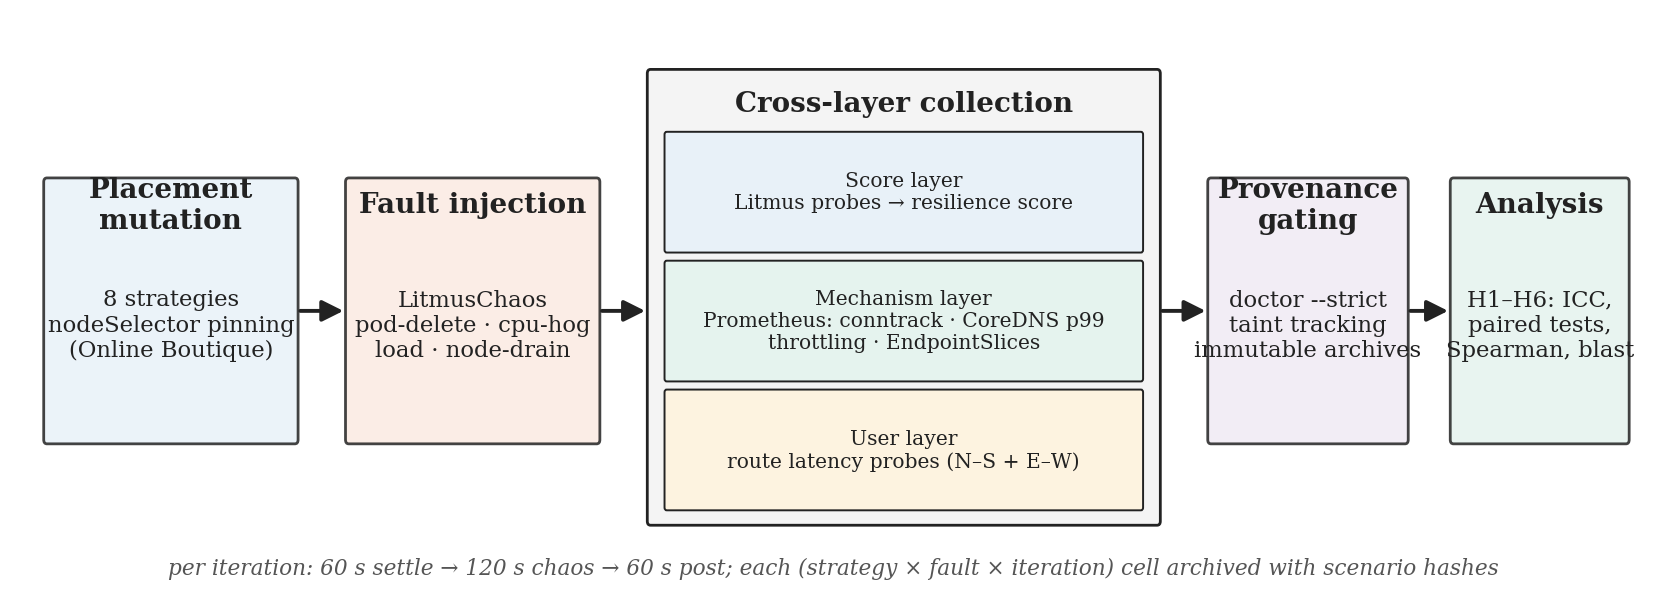
\includegraphics[width=\textwidth]{fig-01-workflow.png}
  \caption{\textbf{ChaosProbe experiment workflow} --- placement mutation $\rightarrow$
    settle $\rightarrow$ load + chaos injection $\rightarrow$ post-chaos probing $\rightarrow$ aggregation $\rightarrow$
    provenance stamping $\rightarrow$ archive.}
  \label{fig:workflow}
\end{figure}

Each experiment iteration follows the pipeline in Figure~\ref{fig:workflow}. The placement
mutator first realizes the strategy under test and waits for the deployment
to settle; the load generator and the continuous probers then start, the
fault is injected and held for the chaos window, and probing continues
through a post-chaos phase so recovery is captured. The per-iteration data is
aggregated into a per-strategy summary, stamped with the run's provenance
manifest, and --- for campaign sessions --- archived as the citable artifact.
The chaos runner, the load generator, and every continuous prober run in
parallel during the chaos window; their outputs are joined only after the
iteration ends, so no prober's sampling cadence depends on another's.

\section{Architecture}\label{sec:architecture}

The implementation is a single Python package whose top-level modules map
one-to-one onto the responsibilities below: \texttt{placement/} (strategies and
the mutator), \texttt{chaos/} (the LitmusChaos runner), \texttt{orchestrator/} (phasing,
readiness, recovery, diagnostics), \texttt{metrics/} and \texttt{collector/} (the probers
and result collection), \texttt{loadgen/} (Locust), \texttt{storage/} (Neo4j),
\texttt{output/} (summary generation, charts, reports), and \texttt{commands/} (the CLI
surface). The description below follows that layout, so each architectural
claim in this chapter is checkable against a named module.

\textbf{CLI} (\texttt{chaosprobe}). The command-line interface is the framework's only
entry point, organized around the experiment lifecycle: \texttt{init} installs
cluster infrastructure (LitmusChaos, Prometheus, Neo4j, the in-cluster
registry), \texttt{run} executes a strategy $\times$ fault $\times$ iteration matrix, and the
analysis commands --- \texttt{doctor}, \texttt{stats}, \texttt{power}, \texttt{report}, \texttt{recommend},
\texttt{summarize}, \texttt{inspect}, \texttt{diff}, \texttt{export} --- consume the resulting
\texttt{summary.json} without touching the cluster. A \texttt{cluster vagrant} command
group manages the Vagrant-provisioned local cluster (\S\ref{sec:environment}), and archiving a finished
run into the citable \texttt{dist/} store is performed by the committed
\texttt{scripts/archive\_run.py}. Two properties matter methodologically. First,
\texttt{run} is \textbf{self-healing}: it verifies and reinstalls missing infrastructure
before each invocation, so experiments are re-entrant and a campaign session
never silently runs against a half-provisioned cluster. Second, the analysis
commands are pure functions of the stored output: every statistic in Chapter
\ref{ch:results} can be recomputed from an archived \texttt{summary.json} without cluster access.

\textbf{Placement mutator \& strategies.} Placement is manipulated at the
deployment level: the mutator (\texttt{placement/mutator.py}) patches each
deployment's \texttt{nodeSelector} to pin services to nodes, realizing eight
strategies defined in \texttt{placement/strategy.py} --- \texttt{baseline} (a no-fault
control that leaves placement and injects nothing), \texttt{default} (the unmodified
Kubernetes scheduler), \texttt{colocate} (all services on the target's node),
\texttt{spread} (services distributed across workers, deterministic per-service
pinning), \texttt{adversarial} (a worst-fit resource hotspot), \texttt{random} (seeded, so
reproducible), \texttt{best-fit} (bin-packing onto the fewest nodes), and
\texttt{dependency-aware} (a BFS partition of the service dependency graph).
These eight are the framework's general-purpose placement primitives; the
pre-registered study does not select among them directly but drives placement
through the two continuous knobs --- the cross-node fraction $f$ and the
replication degree $r$ --- that \S\ref{sec:scheduler-lineage} anchors to the
scheduler literature, with the solver realizing the per-service pinning that hits
each target $f$. Because a \texttt{nodeSelector} is a
request to the scheduler, not a guarantee of the realized state, the mutator
verifies the outcome: each iteration records per-service
\textbf{\texttt{placementMatchRates}} --- the fraction of pods that actually landed where
the strategy intended --- so mismatched iterations are visible to the analysis
rather than silently polluting it (\S\ref{sec:threats-table}). Manipulating $f$
at one replica per service is a scoping decision with consequences the thesis
returns to repeatedly: it cleanly varies \emph{between-service} topology, while
\emph{within-service} replication is exercised only by the $r$ knob in H3's
node-drain campaign --- multi-replica anti-affinity beyond that regime is out of
scope (\S\ref{sec:generalizes}, \S\ref{sec:future-work}).

\textbf{LitmusChaos runner.} Fault injection is delegated to LitmusChaos: the
runner (\texttt{chaos/runner.py}) saves, triggers, and polls ChaosEngine experiments
(\texttt{pod-delete}, CPU/memory hogs, \texttt{node-drain}) through the ChaosCenter GraphQL
API, wrapping each in the settle $\rightarrow$ chaos $\rightarrow$ post phasing that gives the
probers stable pre- and post-fault baselines. The aggregate resilience
score of \S\ref{sec:three-layer} is computed from these experiments' probe verdicts ---
including command probes whose images \texttt{run} builds and pushes to an
in-cluster registry --- which is why the score's failure modes track the
probes' own dependencies on cluster health (\S\ref{sec:decoupling}). The runner carries two pieces
of hardening that campaign-scale operation forced. Injection attempts retry
with best-attempt quality handling: a transient Litmus failure retries, and
if no attempt is fully clean the best attempt is kept \emph{and marked}, so the
data-quality gate (\texttt{doctor}) can taint or exclude the iteration instead of
the run aborting or the defect passing unnoticed. And destructive faults have
cleanup guards --- after \texttt{node-drain}, the runner uncordons any node left
cordoned by a failed experiment teardown, because a leaked cordon would
silently change the cluster available to every subsequent iteration.

\textbf{Orchestration, readiness gates, and recovery measurement.} Between the
mutator and the runner sits the orchestrator, which owns the property the
statistics of Chapter~\ref{ch:methodology} quietly depend on: that every iteration of every
strategy is measured under the same protocol. A pre-flight module validates
the scenario and cluster state before each iteration; readiness gates hold
the iteration until the target pod is running, the application answers
end-to-end, and a warmup period has passed --- so the pre-chaos baseline is a
settled system, not a deployment still converging from the previous
placement mutation. Timing arithmetic derives the probe windows from the
declared chaos duration, so settle, chaos, and post-chaos phases are
identically proportioned across strategies and sessions. A recovery watcher
follows the target deployment's pod lifecycle through the kill cycle,
recording deletion, scheduled, and ready timestamps --- the source of the
recovery times used in the availability analysis. When a Litmus probe returns
an \texttt{Unknown} verdict, a diagnostics module captures the cluster state at
that moment, which is how the study can assert \emph{why} the Litmus score is
unusable under node drain --- the reason H3's availability is measured from
EndpointSlice troughs (\S\ref{sec:h3}) --- rather than merely observing that it
is.

\textbf{Probers (cross-layer).} The measurement design of \S\ref{sec:three-layer} is realized by a
set of continuous probers that run concurrently through every iteration. The
\emph{Prometheus mechanism prober} samples kernel- and infrastructure-layer
signals via PromQL: \texttt{conntrack\_entries\_per\_node} (the H2 signal), CoreDNS
request-duration tails, TCP retransmits, and CPU throttling; kube-proxy's own
network-programming-latency metric is queried but recorded as uncollected on
this cluster (\S\ref{sec:threats-table}) --- the framework's \texttt{metricAvailability} map distinguishes
``not collected'' from ``collected zero'' precisely so such gaps cannot
manufacture fake values. The \emph{route latency prober} measures the user layer:
per-route p50/p95/p99 and error rate against the application's HTTP routes,
with routes classified as fault-\textbf{dependent} (they touch the chaos target)
or \textbf{control} (they do not) --- the confound-control split that H3 and H4
rest on. \emph{Redis, disk, and resource probers} track application state, I/O,
and node/container resource trajectories. Finally, an \emph{EndpointSlice
snapshotter} records per-service ready-endpoint counts every 15 s through
the chaos window; its outage troughs are the basis of the trough-depth
blast-radius metric H3 uses, which deliberately bypasses both the score and the
route layer (under a node drain, every Litmus probe returns \texttt{Unknown} and
the score is unusable --- \S\ref{sec:h3}).

\textbf{Load generation.} User traffic is generated by Locust profiles against
Online Boutique's user-facing routes: a steady profile (50 users) provides
background traffic for churn experiments, and a 200-user spike profile
provides elevated user load during the chaos window. The load generator runs in
parallel with the probers throughout the chaos window, so the route prober
measures latency under the same traffic the fault perturbs.

\textbf{Storage.} Each run emits structured per-iteration JSON aggregated into a
per-strategy \texttt{summary.json} (output schema 2.0.0) --- the single artifact all
analysis consumes --- and writes a \textbf{Neo4j graph} of services, dependency
edges, and per-iteration pod$\rightarrow$node placements. For most of the study the
graph is storage; the cross-node fraction knob makes it \textbf{analytically
load-bearing}: the cross-node call fraction $f$ --- the placement knob the study
manipulates --- is computed by joining the graph's inter-service edges with the
recorded \texttt{podPlacements}, so each placement's realized $f$ is known
\emph{before any chaos is injected} and depends on the graph being a faithful
model of the application's call structure. The \texttt{summary.json}
itself is organized for exactly the analyses Chapter~\ref{ch:results} performs: per
strategy it carries the per-iteration scores, probe verdicts, recovery
timings, placement match rates, the per-route latency/error aggregates
split by dependent-vs-control classification, the mechanism metric
time-series summaries with their \texttt{metricAvailability} flags, and the
\texttt{routeViewAggregate} from which the east-west inter-service tails of H1
and H4 are read. Nothing downstream re-queries the cluster; the file is the
experiment's complete, self-describing record.

\textbf{Analysis commands.} Downstream analysis is split between the CLI and
committed campaign scripts. \texttt{doctor} is the data-quality gate: it checks
per-iteration completeness, probe verdicts, and placement match, and in
\texttt{--strict} mode additionally refuses runs with incomplete provenance (\S\ref{sec:provenance}).
\texttt{stats} computes pairwise strategy statistics; \texttt{report} renders
HTML/Markdown reports; \texttt{recommend} summarizes the per-strategy comparison.
The campaign-level numbers in Chapter~\ref{ch:results} come from dedicated scripts ---
\texttt{scripts/c1\_h1\_trend.py} (H1, Page's $L$ dose-response),
\texttt{c3\_h2\_dns.py} (H2, placement + DNS), \texttt{c2\_h3\_anova.py} (H3, ART
ANOVA replication rescue), the frontier driver (H4),
\texttt{scorecard.py} (H5 layered-scorecard ICC), \texttt{holm\_family.py} (the
family Holm correction), and \texttt{campaign\_status.py} (session bookkeeping)
--- each committed in the
repository, so every quoted figure names the code path that produced it.

Three design principles cut across these components and are worth stating
once. First, \textbf{measurement is separated from judgment}: the probers record
what happened --- including taints, partial data, and \texttt{Unknown} verdicts ---
and the decision about whether an iteration's data is usable belongs to
\texttt{doctor}, applied after the fact under explicit, versioned rules. Nothing
in the collection path drops inconvenient data. Second, \textbf{absence is
recorded, not interpolated}: the \texttt{metricAvailability} map exists because
the most dangerous failure mode of a metrics pipeline is a missing query
that reads as zero; a metric ChaosProbe could not collect is stored as
uncollected, and the analysis scripts treat it as such. The kube-proxy
network-programming-latency metric is the live example --- queried, never
scraped on this cluster, and therefore cited in this thesis only as
conceptual anchoring for the mechanism, never as data (\S\ref{sec:threats-table}). Third,
\textbf{every number is regenerable}: the chain from CLI flags to scenario YAML
to \texttt{summary.json} to analysis script is deterministic given the archived
inputs, which is what allows Appendix~\ref{app:provenance} to function as a claims$\rightarrow$runs
mapping rather than a bibliography of irreproducible measurements.

The framework's limitations are part of its honest description. Placement
is mutated at deployment level with \texttt{nodeSelector}, which is what makes
the realized placement verifiable, but also what restricts the study to
between-service topology --- per-service replica anti-affinity is out of
reach of the current mutator, a boundary that shapes the future-work
design in \S\ref{sec:future-work}. The probers sample at fixed cadences (EndpointSlice
snapshots every 15 s), so sub-cadence transients are invisible; the
blast-radius troughs (H3) are well above this resolution, but finer-grained
availability dynamics would need a faster snapshotter. And the framework
measures one cluster at a time: nothing in the design prevents running the
same campaign on different infrastructure, but the cross-environment
comparison itself is future work, not a shipped feature.

\section{Provenance capture}\label{sec:provenance}

Every run is stamped with a manifest (\texttt{artifact-manifest.json}) carrying:

\begin{itemize}
\item \textbf{scenario SHA-256 hashes} (the exact fault YAML injected),
\item \textbf{batch/day IDs} and run ID,
\item \textbf{kube-proxy mode and conntrack settings} (mode, \texttt{maxPerCore}, \texttt{min},
  TCP timeouts) --- required because the H2 mechanism is version- and
  mode-sensitive,
\item \textbf{git commit} (+ dirty flag) of the framework code,
\item \textbf{environment fingerprint}: Kubernetes server version, container runtime,
  node OS, CNI hint, namespace, strategy/fault matrix, iteration count.
\end{itemize}

\texttt{doctor --strict} refuses a run whose provenance is incomplete or whose
scenario hashes drift; \texttt{scripts/archive\_run.py} banks the run under
\texttt{chaosprobe/dist/} as the citable artifact (Appendix~\ref{app:provenance}).

Provenance is a first-class feature of the framework, not packaging
convenience, for three reasons. First, the claims demand it: the H2
mechanism is sensitive to the Kubernetes version, the kube-proxy mode, and
the kernel's conntrack configuration (\S\ref{sec:h2-mechanism} --- upstream conntrack handling
changed materially across v1.31--v1.32), so a conntrack-flush number quoted
without its environment fingerprint is not interpretable, let alone
reproducible. The manifest pins exactly the parameters on which the
mechanism's scope depends.

Second, weak provenance has an empirical cost. An early, weakly-provenanced
pilot run --- with untracked working-tree changes and incomplete metadata ---
produced a striking user-layer number that did not survive: when the
measurement was repeated under \texttt{doctor}-gated, strict-clean runs, the
user-layer effect collapsed and only the mechanism-layer effect persisted. Had
the un-gated pilot been quoted, a headline result would have been an artifact of
an unreproducible run state. The lesson is institutionalized as the campaign
rule that no number is quoted from a run failing \texttt{doctor --strict}, and as
the manifest's dirty flag, which makes an uncommitted-code run permanently
visible as such.

Third, the external advisory review of this work flagged missing raw
artifacts as a blocker: findings quoted in prose with no bankable evidence
trail. The archive pipeline answers that structurally rather than
procedurally --- \texttt{scripts/archive\_run.py} packages each run's \texttt{summary.json},
per-strategy data, charts, and manifest, with per-file SHA-256 hashes, under
\texttt{chaosprobe/dist/}, and Appendix~\ref{app:provenance} maps every claim in Chapter~\ref{ch:results} to the
archives that carry it. The provenance chain is thus verifiable end to end:
from a number in this document, to a named archive, to hashed data files, to
the exact scenario YAML and code commit that produced them.

% Ported from thesis/04-methodology.md — wording unchanged.
\chapter{Methodology}\label{ch:methodology}

% This chapter substantiates contribution claim 3 (the provenance-gated
% campaign protocol) and defines the measurement design behind H1–H6.

This chapter defines how the research question of \S\ref{sec:rq} is turned into
measurements: the three-layer measurement design (\S\ref{sec:three-layer}), the three fault
classes and the negative findings that shaped their selection (\S\ref{sec:fault-classes}), the
multi-session campaign protocol that is itself a contribution (\S\ref{sec:campaign}), the
statistical methods (\S\ref{sec:statistics}), and the pinned cluster environment every claim
is scoped to (\S\ref{sec:environment}).

\section{Three-layer measurement design}\label{sec:three-layer}

Each experiment is measured at three layers that need not agree --- the study's
unit of explanation is \emph{which layer moves}:

\begin{enumerate}
\item \textbf{Aggregate score} --- the probe-based resilience score (the industry-style
   single number; H1 audits its reliability).
\item \textbf{Mechanism metrics} --- kernel/network signals: conntrack entries per
   node, CoreDNS tail latency, TCP retransmits, CPU throttling, east-west
   inter-service route tails (H2, H4, H5).
\item \textbf{User-visible routes} --- per-route tail latency and error rate, with a
   built-in \textbf{dependent-vs-control confound check}: \emph{dependent} routes
   touch the chaos target (\texttt{productcatalogservice}), \emph{control} routes do
   not, so a genuine fault-specific effect must show on dependent routes
   \emph{beyond} the control route's run-level drift (H3, H4).
\end{enumerate}

The confound-controlled user layer is the difference between ``correlates
with the run'' and ``caused by the fault path'', and it is load-bearing for
every user-layer statement in this thesis. The threat it addresses is
run-level drift: on a small virtualized cluster, entire runs are slower or
faster than each other for reasons unrelated to the fault --- host load,
cache state, background reconciliation. Any mechanism metric measured in a
slow run will correlate with any latency measured in the same slow run, so
a naive correlation between mechanism and user outcome is uninterpretable.
The control routes break this degeneracy. Because they ride the same run
but do not traverse the killed service, they carry the run-level drift and
nothing else; a genuine propagation from mechanism to user must therefore
show an association on the dependent routes that is both significant and
clearly in excess of the control routes' association. The diagnostic also
works in reverse, and Chapter~\ref{ch:results} uses it that way: when the \emph{control} route
correlates with the mechanism more strongly than the dependent route does
(H3: $\rho = 0.29$ on control vs 0.07 on dependent), the association is
positively identified as a run-level confound rather than merely failing
significance. A within-run rank correlation --- computed inside each run,
where run-level drift is constant by construction --- confirms the read.

Each layer is read by a different instrument, and the instruments fail
independently --- which is itself informative. The aggregate score derives
from LitmusChaos probe verdicts; the mechanism layer from PromQL samples of
kernel and infrastructure metrics; the user layer from the route prober's
active HTTP measurements under Locust traffic. We deliberately \emph{audit} the
industry-style aggregate score rather than redesigning it: H1's question is
whether the instrument operators currently have can support the ranking
task they implicitly use it for, and answering that requires measuring the
score as-is, with its reliability quantified rather than assumed. The
layered design also means no single instrument's blind spot is fatal --- a
property Chapter~\ref{ch:results} exercises three times, when the score turns out noisy
under churn, saturated under load, and unusable under node drain, while
the other two layers keep reporting.

\section{Fault classes}\label{sec:fault-classes}

\begin{center}
\begin{tabular}{p{0.17\textwidth}p{0.3\textwidth}p{0.42\textwidth}}
\toprule
\textbf{Class} & \textbf{Fault} & \textbf{What it perturbs} \\
\midrule
\textbf{Churn} & \texttt{pod-delete} & Endpoint/identity turnover: EndpointSlice, conntrack, DNS reconvergence \\
\textbf{Load contention} & sustained 200-user Locust spike (near-no-op hog placeholder) & Genuine resource contention --- the regime hogs cannot create here (Appendix~\ref{app:negative}) \\
\textbf{Node failure} & \texttt{node-drain} of the target's node & Availability: blast radius and rescheduling \\
\bottomrule
\end{tabular}
\end{center}

The three classes were chosen to perturb three distinct subsystems, so that
``does placement matter?'' gets a per-mechanism answer rather than a pooled
one. Churn (\texttt{pod-delete}) destroys and recreates a service's only replica:
the pod's identity, IP, and endpoints turn over, and the cluster's
networking state --- EndpointSlice membership, conntrack entries, DNS answers
--- must reconverge. This is the disruption window the Kubernetes
SIG-Scalability community tracks with its own network-programming-latency
SLO \citep{k8scommunity-netslo}.
Load contention drives the application against its resource limits while
fully available, making latency --- not availability --- the outcome under
stress. Node failure (\texttt{node-drain}) removes a whole failure domain, making
availability the outcome and blast radius the natural metric.

The composition of this fault matrix is itself an empirical result, and we
present the dead-ends as methodological findings because they show that the
\emph{obvious} contention experiments probe the wrong layer on clusters of this
class (Appendix~\ref{app:negative} gives the full autopsies). The standard chaos catalog
offers CPU and memory hog faults as the contention instruments, and all of
them null out here for documented, mechanistic reasons. \texttt{pod-cpu-hog} is
capped by the CFS quota at the victim container's own 200m CPU limit: the
stressor consumes the victim's budget, every other pod is untouched, the
application stays up, and the resilience score sits at $\approx$ 100. \texttt{node-cpu-hog}
loads the node, but Kubernetes CPU \emph{requests} guarantee the lightweight
application pods their shares, so they remain responsive. \texttt{node-memory-hog}
fails more subtly: its stress helper computes its target against node
capacity, clamps to allocatable, and on an already-utilized 4 GiB worker
becomes the kubelet's \emph{first eviction victim} --- it self-evicts before any
application pod feels pressure (confirmed against the \texttt{litmus-go} source ---
\href{https://github.com/litmuschaos/litmus-go/blob/master/chaoslib/litmus/node-memory-hog/lib/node-memory-hog.go}{\texttt{calculateMemoryConsumption}}
applies the percentage to node \emph{capacity}, clamps to allocatable, and ignores
in-use memory; a
100\%-consumption probe produced zero MemoryPressure, OOM, or app-pod
evictions). The consequence is the design above: genuine contention must
come from \emph{load} --- the 200-user Locust spike, under which the application is
actually resource-bound --- with the hog fault reduced to a near-no-op
placeholder so the experiment pipeline's phasing is preserved. Studies that
report ``no placement effect under CPU hogs'' without this analysis would be
reporting a property of the fault, not of placement.

A terminological note: the \emph{churn-versus-contention} distinction used
throughout this thesis is our own framing, not an established taxonomy ---
our literature search found no peer-reviewed work that classifies
\texttt{pod-delete} as a churn fault distinct from contention faults (\S\ref{sec:tail-latency}). We
adopt it because the mechanisms differ categorically: a churn fault
perturbs \emph{identity and networking state} (endpoints, conntrack, DNS) and
its user-visible damage is bounded by availability dynamics, while a
contention fault perturbs \emph{resource budgets} and its damage is latency
under load. The negative findings above are what the distinction predicts:
faults marketed as contention instruments that cannot actually create
contention on this cluster produce null results at every layer.

\section{Campaign design}\label{sec:campaign}

\begin{itemize}
\item \textbf{Unit of analysis: the session.} One \texttt{run} invocation on one git commit =
  one independent session. The primary campaign is \textbf{7 sessions (s01--s07)},
  each all 8 strategies $\times$ $i = 3$ (147 churn iterations total), banked under
  \texttt{campaign-results/} and archived to \texttt{dist/}.
\item \textbf{Gating.} Every session must pass \texttt{doctor --strict} (provenance + data
  quality) before its numbers are used; failed/partial sessions are discarded,
  not patched.
\item \textbf{Blocking \& controls.} \texttt{baseline} is a no-fault control; strategy order is
  fixed within a session; batch/day IDs allow day-level blocking; pre/post
  snapshots bound run drift.
\item \textbf{Replication discipline.} Mechanism claims require direction-consistency
  across sessions (H2: 7/7); user-layer claims require survival across
  independent batches (H4's did not, and is therefore not claimed).
\end{itemize}

The session is the campaign's unit of analysis because it is the unit at
which the dominant noise operates. H1's variance decomposition shows that
37.6\% of score variance is run-to-run: whole invocations differ from each
other more than strategies differ within an invocation. Pooling iterations
across runs as if they were independent would therefore understate the
uncertainty of every between-strategy comparison. Treating the session as
the replicate --- and requiring effects to reproduce \emph{across} sessions, not
merely within one --- is the conservative response.

We state the independence structure plainly. Sessions are independent
\emph{invocations}: each is a separate \texttt{run} execution, launched at a different
time, with its own settle phases, its own realized placements, and its own
draw of environmental conditions. Each session ran on a single framework
commit throughout, but sessions are not all on \emph{distinct} commits --- s02 and
s03 share one commit, and s04--s07 share another (Appendix~\ref{app:provenance} lists the
mapping). Independence is therefore per invocation and day, not per code
version; what the single-commit rule guarantees is that no session mixes
code versions internally, which was a real defect of the pre-campaign
pooled run-set (16 runs across heterogeneous code versions and probe
counts, retained only as a pilot tier).

Two further design choices bound what the campaign can and cannot absorb.
Strategy order is fixed within each session, so any slow within-run drift
loads onto the same strategy positions in every session --- a conservative
choice that converts a potential random confound into a constant one, at
the cost of not being able to separate order effects from strategy effects
within a single session (across sessions, the direction-consistency
requirement defends against this). And the \texttt{baseline} cell --- placement
untouched, no fault injected --- runs in every session as a no-fault control,
bounding what the score and the probers report when nothing is done.

The gate deserves its own paragraph because it is the protocol's teeth.
\texttt{doctor --strict} is an automated check applied to a finished run before
any of its numbers may be quoted: it verifies per-iteration data
completeness, probe verdicts, placement match rates, and taint status, and
in strict mode additionally the provenance fingerprint --- scenario SHA-256
hashes against the committed YAML, kube-proxy mode and conntrack settings,
git commit and dirty flag, and the environment manifest (\S\ref{sec:provenance}). The rule
attached to it is \emph{discard, not patch}: a session that fails the gate is
excluded whole, never repaired by dropping its bad iterations and keeping
the rest, because selective repair is a selection effect on exactly the
noise H1 measures. The rule has been exercised, not merely stated --- the
original H4 pilot, whose user-layer effect was the most striking number in
the study at the time, was discarded for dirty provenance and replaced
with two clean batches, which is how the study learned that the effect
does not replicate (\S\ref{sec:h4}).

\section{Statistics}\label{sec:statistics}

\begin{itemize}
\item \textbf{Variance partition} of the per-iteration score into between-strategy /
  run-to-run / iteration components; \texttt{ICC\_strategy} with a \textbf{cluster
  bootstrap} 95\% CI (resampling sessions, preserving within-session
  correlation).
\item \textbf{Paired Wilcoxon signed-rank + exact sign tests} across sessions for the
  focal spread-vs-colocate mechanism contrast (H2).
\item \textbf{Spearman rank correlations} for mechanism$\rightarrow$outcome (H3) and
  predictor$\rightarrow$tail (H5), plus \textbf{TOST equivalence testing} to support
  ``decoupled'' as a positive statistical statement rather than absence of
  evidence.
\item \textbf{ART ANOVA} (aligned-rank transform) as a nonparametric factorial helper
  where interactions are examined (e.g.\ node-drain analyses).
\item \textbf{Power analysis} for H1: Cohen's $d$ of the focal contrast $\rightarrow$ iterations
  needed for 80\% power ($\alpha = .05$, two-sided), and the minimum detectable
  effect at the $n$ actually run.
\end{itemize}

\textbf{Model and notation.} Let $y_{sri}$ be the aggregate score of
iteration $i$ of strategy $s$ in session (run) $r$. H1's decomposition uses
the crossed random-effects model
\[
  y_{sri} = \mu + \alpha_s + b_r + \varepsilon_{sri},
\]
with $\alpha_s$ the strategy effect (variance $\sigma^2_\alpha$),
$b_r$ the session effect ($\sigma^2_b$), and $\varepsilon_{sri}$ the
residual iteration noise ($\sigma^2_\varepsilon$). The quantity H1 reports is the
intraclass correlation of strategy,
\[
  \mathrm{ICC}_{\mathrm{strategy}} = \sigma^2_\alpha \,/\, (\sigma^2_\alpha + \sigma^2_b + \sigma^2_\varepsilon),
\]
the fraction of total score variance attributable to which strategy was
running --- the ceiling on how well \emph{any} ranking procedure based on this
score can do. The components are estimated from the 147 campaign iterations
by the committed \texttt{scripts/score\_variance.py}; the campaign estimates are
$\sigma^2_\alpha : \sigma^2_b : \sigma^2_\varepsilon = 3.3\% : 37.6\% : 59.1\%$
(\S\ref{sec:h1}).

\textbf{Cluster bootstrap, worked.} A naive bootstrap over the 147 iterations
would treat them as exchangeable, which they are not --- iterations within a
session share the session effect $b_r$. The cluster bootstrap
resamples at the level the dependence lives: draw 7 sessions \emph{with
replacement} from \{s01\ldots s07\} (a resample might be s02, s02, s04, s05, s05,
s07, s07), keep every drawn session's iterations intact, recompute
$\mathrm{ICC}_{\mathrm{strategy}}$ on the resampled data, repeat, and take the 2.5th and
97.5th percentiles of the resulting distribution as the 95\% CI. This
preserves within-session correlation exactly and yields the interval
[0.014, 0.178] reported in \S\ref{sec:h1} --- wide, as expected with 7 clusters, but
bounded well below the range where score-based ranking would be feasible.

\textbf{Paired tests across sessions (H2).} The focal mechanism contrast is
evaluated at session level: for each session, the median conntrack flush of
\texttt{spread} minus that of \texttt{colocate}, giving 7 paired differences. The exact
sign test asks only for direction (all 7 positive: $p = 2 \times 0.5^7 =
0.0156$ two-sided); the Wilcoxon signed-rank test adds magnitude ordering
($W = 0$, $p = 0.0225$). Both are reported because with $n = 7$ the sign test
is the assumption-free floor and Wilcoxon the more powerful companion.

\textbf{Correlation, equivalence, and the factorial helper.} Associations between
layers (H3) and between predictor and outcome (H5) use Spearman rank
correlation, which is invariant to the monotone-but-nonlinear scales these
metrics live on. For H3, a non-significant correlation alone would be
absence of evidence; the decoupling claim is therefore additionally
supported by TOST (two one-sided tests) equivalence testing, which asks
whether the association is \emph{demonstrably small}, not merely undetected
\citep{schuirmann1987equivalence,lakens2017equivalence}.
We import the procedure from biostatistics deliberately: no native
equivalence-testing precedent exists in the systems-performance venues we
searched, and the nearest peer-reviewed computer-science precedent for
affirmatively accepting practical equivalence is the region-of-practical-equivalence
analysis of Benavoli et al.\
\citep{benavoli2017time}. TOST
requires a pre-declared smallest effect size of interest: ours is
$|\rho| = 0.3$ --- the conventional small-correlation boundary --- fixed in the
committed analysis code (\texttt{tost\_equivalence\_correlation}, default
\texttt{sesoi = 0.3}) before the campaign ran, not chosen after seeing the data.
Where factorial structure is examined (e.g.\ strategy $\times$ phase in the
node-drain analyses), the aligned-rank-transform ANOVA provides a
nonparametric interaction test. \textbf{Power analysis} closes the H1 argument:
from the focal contrast's Cohen's $d = 0.46$, the standard two-sample
calculation gives $\approx$ 73 iterations per strategy for 80\% power at $\alpha = .05$
two-sided; inverting it at the $n = 3$ per session actually run gives a
minimum detectable effect of 2.29 pooled standard deviations --- about 51
score points, larger than any gap that exists in the data (\S\ref{sec:h1}).

The argument \emph{shape} follows Maricq et al.\ (OSDI 2018) --- quantify the
environment's variability, then prescribe what repetition can and cannot
detect --- with the precision note that their CONFIRM uses nonparametric
CI-width stopping, not formal power analysis. Distribution-first reporting
follows Hoefler \& Belli (SC 2015): Chapter~\ref{ch:results} reports medians, tails, and
intervals, not bare means, and the nonparametric toolkit above is the
default throughout.

\section{Cluster environment}\label{sec:environment}

% Values below are from the archived manifests (dist/*/artifact-manifest.json)
% — the citable fingerprint. Pin versions; the H2 mechanism is version-sensitive.

\begin{itemize}
\item \textbf{Cluster}: 5-node kubeadm cluster (1 control plane + 4 workers, 4 GiB RAM
  each) on Vagrant-managed KVM/libvirt VMs on a single host.
\item \textbf{Kubernetes v1.28.6} (pinned --- kube-proxy/conntrack behaviour changed
  materially in v1.31--v1.32, see \S\ref{sec:h2-mechanism}), containerd 1.7.11, Ubuntu 22.04.3 LTS
  nodes, Calico CNI.
\item \textbf{kube-proxy mode: \texttt{ipvs}}, conntrack \texttt{maxPerCore} 32768 / \texttt{min} 131072,
  TCP established timeout 24 h, close-wait 1 h --- all archived per run.
\item \textbf{Workload}: Online Boutique (Google Cloud microservices-demo), 10 polyglot
  gRPC microservices + Redis, single replica per service (the regime under
  study), Locust load generator.
\end{itemize}

\begin{center}
\begin{tabular}{lllll}
\toprule
\textbf{Node} & \textbf{Role} & \textbf{vCPU} & \textbf{RAM} & \textbf{OS} \\
\midrule
control plane ($\times$1) & kubeadm control plane & 2 & 12 GiB & Ubuntu 22.04.3 LTS \\
worker ($\times$4) & workload nodes & 2 each & 4 GiB each & Ubuntu 22.04.3 LTS \\
\bottomrule
\end{tabular}
\end{center}

All five VMs run on a single physical host under KVM/libvirt, which makes
host-level interference --- other VMs' scheduling, host I/O, host memory
pressure --- a shared, time-varying influence on every measurement. We treat
this as a property of the environment to be \emph{absorbed by design} rather
than eliminated: it is precisely the noise source that surfaces as the
37.6\% run-to-run variance component in H1, that the session-level campaign
protocol blocks against (\S\ref{sec:campaign}), and that the dependent-vs-control route
split controls for within runs (\S\ref{sec:three-layer}). The environment values above are not
incidental: the H2 mechanism is contingent on the kube-proxy mode (\texttt{ipvs}
here), the conntrack configuration, and the Kubernetes version, all of
which are stamped into every archived run's manifest so that each
mechanism-level claim carries its exact scope (\S\ref{sec:provenance}). What does and does not
port out of this pinned environment is stated once, in \S\ref{sec:generalizes}'s table.

% Ported from thesis/05-results.md — wording unchanged.
\chapter{Results}\label{ch:results}

% Numbers in this chapter are FINAL (post-#245): the 7-session campaign
% (s01–s07) is the primary H1–H3 evidence; the pooled pre-campaign run-set is
% pilot-only. Every number traces to an archived run via Appendix A.
% Wording per scope-of-claims.md.

Reading order: H1 establishes that the aggregate instrument is blind; H2--H4
show placement reproducibly moves mechanism layers that do not reach the
user; H5--H6 locate where placement does bite --- node failure --- as a measured
latency$\leftrightarrow$availability trade-off. The fault-class grouping is churn (H1--H3),
load (H4--H5), node failure (H6).

\begin{figure}[tb]
  \centering
  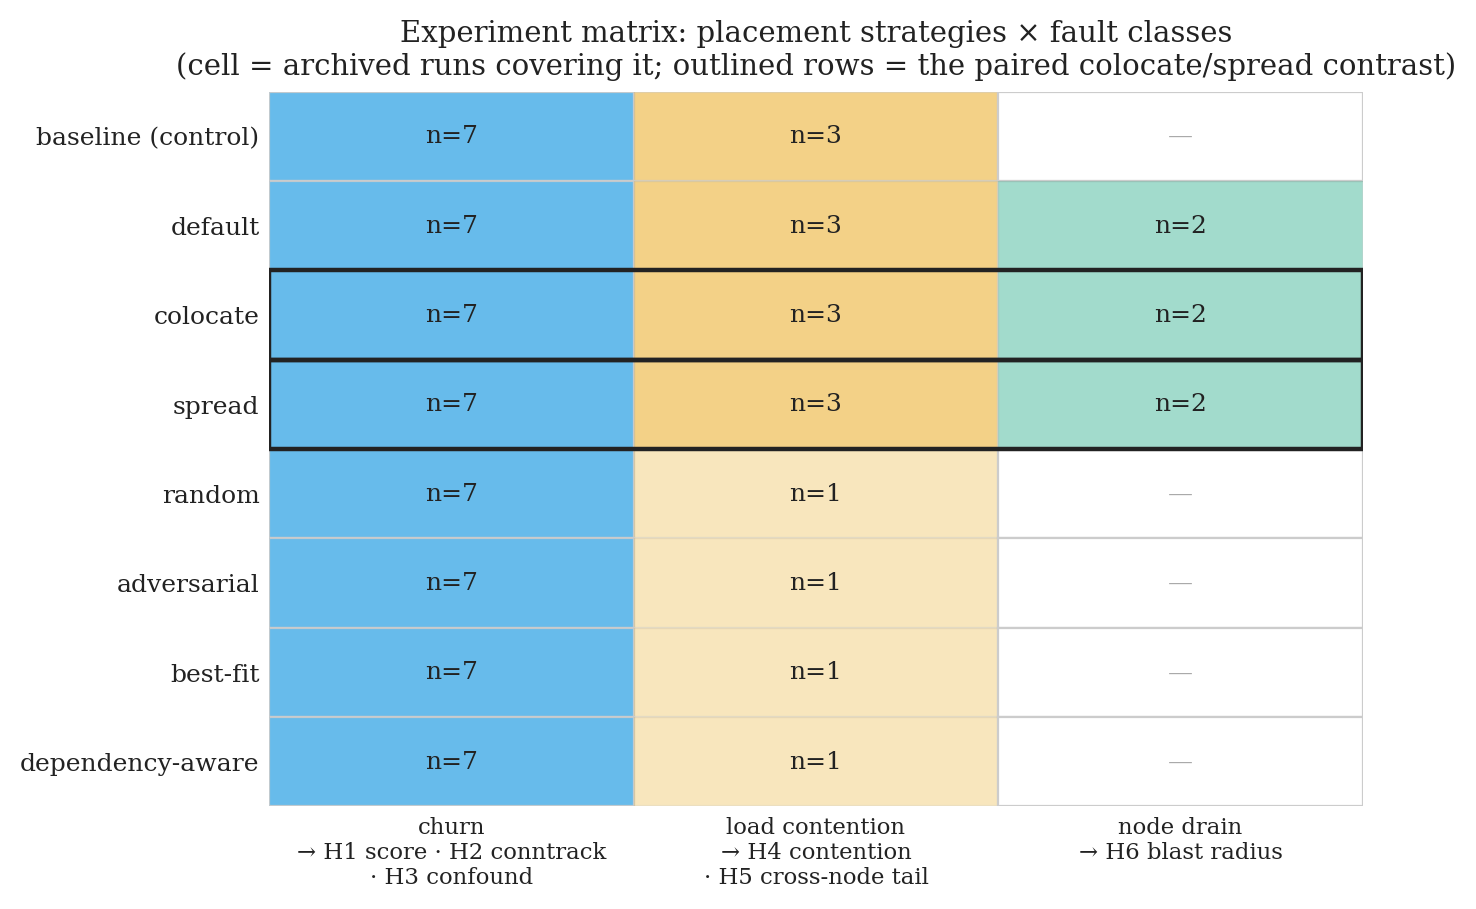
\includegraphics[width=\textwidth]{fig-02-core-matrix.png}
  \caption{The fault-class $\times$ measurement-layer core matrix: which layer
    moves under churn / load / node failure, and whether it reaches the user.}
  \label{fig:core-matrix}
\end{figure}

\section{H1 --- The aggregate score cannot rank placement strategies}\label{sec:h1}

\textbf{Statement.} The probe-based aggregate resilience score does not
reproducibly discriminate placement strategies; between-strategy differences
are a small fraction of total score variance and undetectable at feasible
iteration counts.

\textbf{Result --- supported (7-session campaign, 147 churn iterations).}

\begin{center}
\begin{tabular}{p{0.5\textwidth}p{0.42\textwidth}}
\toprule
\textbf{Quantity} & \textbf{Value} \\
\midrule
\texttt{ICC\_strategy} & \textbf{0.033} (cluster-bootstrap 95\% CI \textbf{[0.014, 0.178]}) \\
Variance partition & between-strategy \textbf{3.3\%} / run-to-run \textbf{37.6\%} / iteration \textbf{59.1\%} \\
Focal contrast (colocate 64.0 vs spread 74.3) & $d = 0.46$ $\rightarrow$ \textbf{73 iterations/strategy} for 80\% power \\
MDE at the $n = 3$ actually run per session & 2.29 sd $\approx$ \textbf{51 score points} --- larger than any gap that exists \\
\bottomrule
\end{tabular}
\end{center}

The earlier pooled run-set (16 mixed-version runs: ICC 0.046, focal $d = 0.06$
needing $\approx$3,982/strategy) read the same way and is retained as the pilot only.

Scope (per \S\ref{sec:positioning}): this is ``cannot \textbf{rank placement strategies under session
variance}'' --- MicroRes's 0.86--0.90 \emph{binary} classification accuracy is a
different task and is not contradicted.

\begin{figure}[tb]
  \centering
  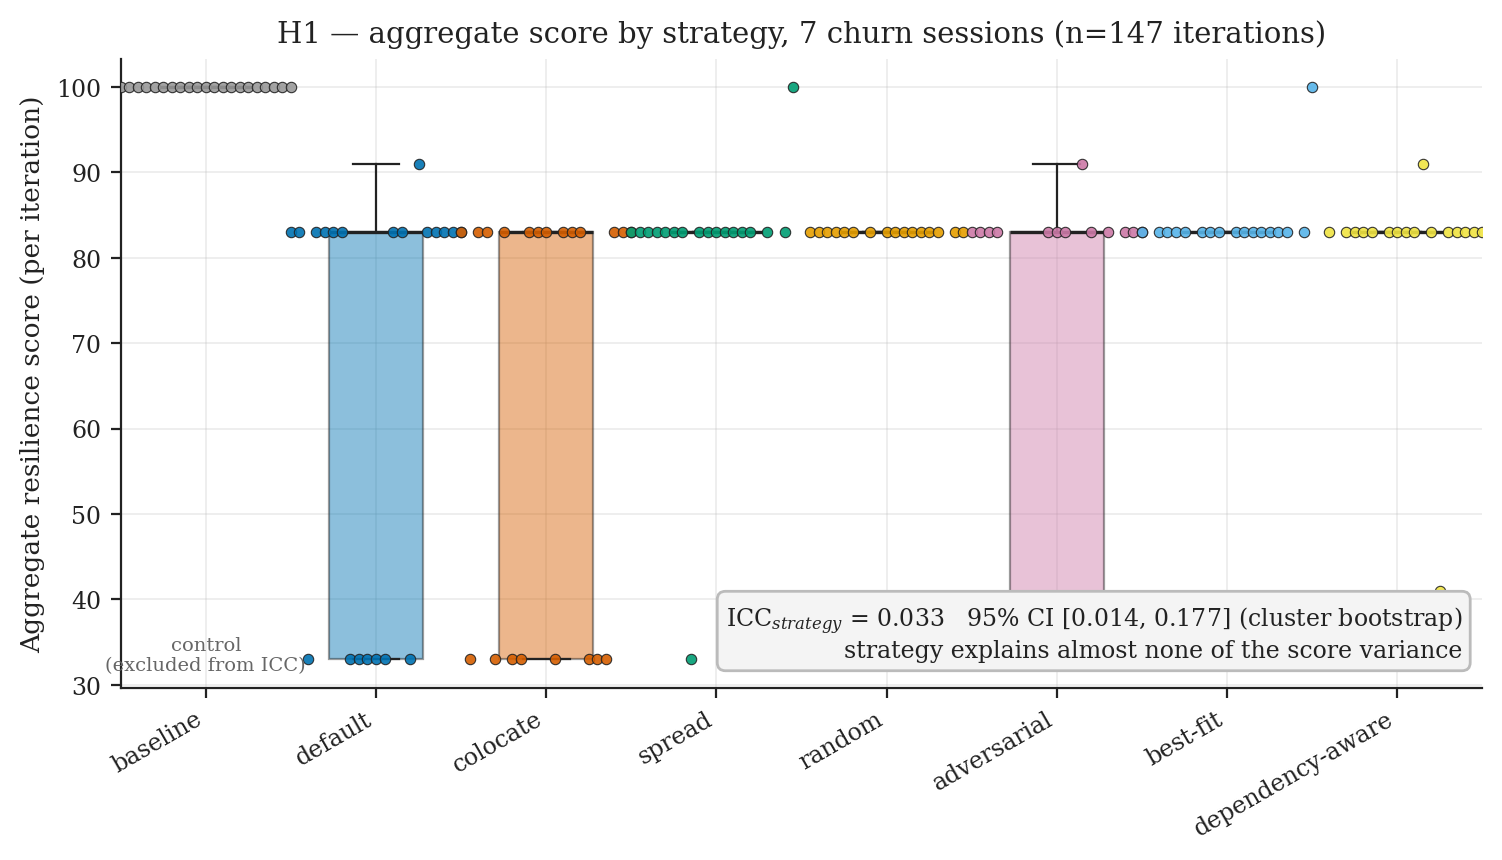
\includegraphics[width=\textwidth]{fig-03-h1-score-distributions.png}
  \caption{Per-strategy score distributions across the seven sessions
    (overlapping spreads, means clustered 64--74).}
  \label{fig:h1-dist}
\end{figure}

\begin{figure}[tb]
  \centering
  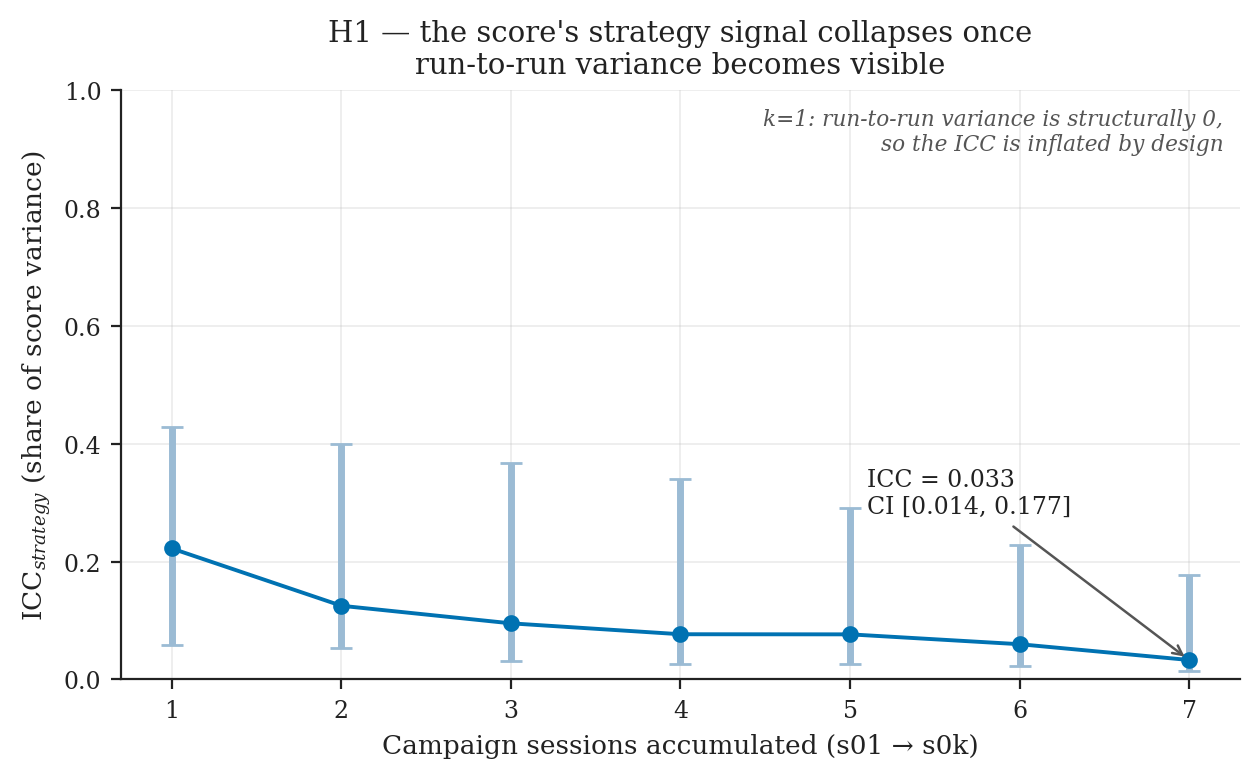
\includegraphics[width=\textwidth]{fig-04-h1-icc-trajectory.png}
  \caption{ICC trajectory as sessions accumulate, 0.222 $\rightarrow$ 0.033
    (run-to-run variance accrues with k).}
  \label{fig:h1-icc}
\end{figure}

\section{H2 --- Placement reproducibly moves a kernel/network reconvergence signature}\label{sec:h2}

\textbf{Statement.} Under churn, spreading the target's dependents across nodes
flushes a large fraction of per-node conntrack state during the kill cycle;
co-location does not.

\textbf{Result --- supported (7/7 sessions).} Median conntrack flush: \texttt{spread}
\textbf{38.5\%} vs \texttt{colocate} \textbf{2.7\%}; \texttt{spread > colocate} in \textbf{7/7} independent
sessions --- \textbf{sign test $p = 0.0156$, paired Wilcoxon $W = 0$, $p = 0.0225$}.
The pooled pilot agreed (36.6\% vs 1.9\%, 16/16 runs). This is the most
reproducible signal in the study.

Secondary, corroborating only: \texttt{colocate} throttles CPU lowest in 6/7
sessions (the pooled pilot had \texttt{best-fit} lower still) --- lead with conntrack.

\textbf{Mechanism --- protocol composition measured.} A dedicated probe (per-node
\texttt{conntrack -L} protocol counts at 5 s intervals through one full kill cycle
under each placement; \S\ref{sec:h2-mechanism}, raw data + chaos-window timestamps in
\texttt{data/conntrack-probe/}) yields three window-robust composition findings:
(1) \textbf{TCP dominates the table under both placements and drops sharply at
the kill cycles in both} (spread 5,935 $\rightarrow$ 4,253, $-$28\%; colocate
4,973 $\rightarrow$ 3,937, $-$21\%) --- kernel-side teardown of flows traversing the killed
pod: kube-proxy has no TCP conntrack-deletion path (\#100698, \#104098;
verified across the $\le$v1.31 exec cleaner and $\ge$v1.32 netlink reconciler), and
close-state conntrack timeouts (10--120 s; \S\ref{sec:h2-mechanism}) expire torn-down flows
within the cycle;
(2) \textbf{the clearly placement-dependent component is UDP (DNS)}: under
steady load \texttt{spread} sustains $\sim$\textbf{4$\times$} more UDP entries than \texttt{colocate}
(chaos-window medians 910 vs 224), consistent with cross-node calls driving
connection churn and DNS re-resolution, and with kube-proxy's documented
UDP-only cleanup (\#48370, \#108523, \#126130; ipvs mode here) having more to
clean under spread; (3) with $i = 1$ and a Locust-ramp-contaminated
baseline, the probe \textbf{cannot apportion the campaign's flush percentages}
between the two paths --- both mechanisms are visible; their shares remain
unquantified. The seven sessions carry the statistics; the probe carries
composition and event timing.

\begin{figure}[tb]
  \centering
  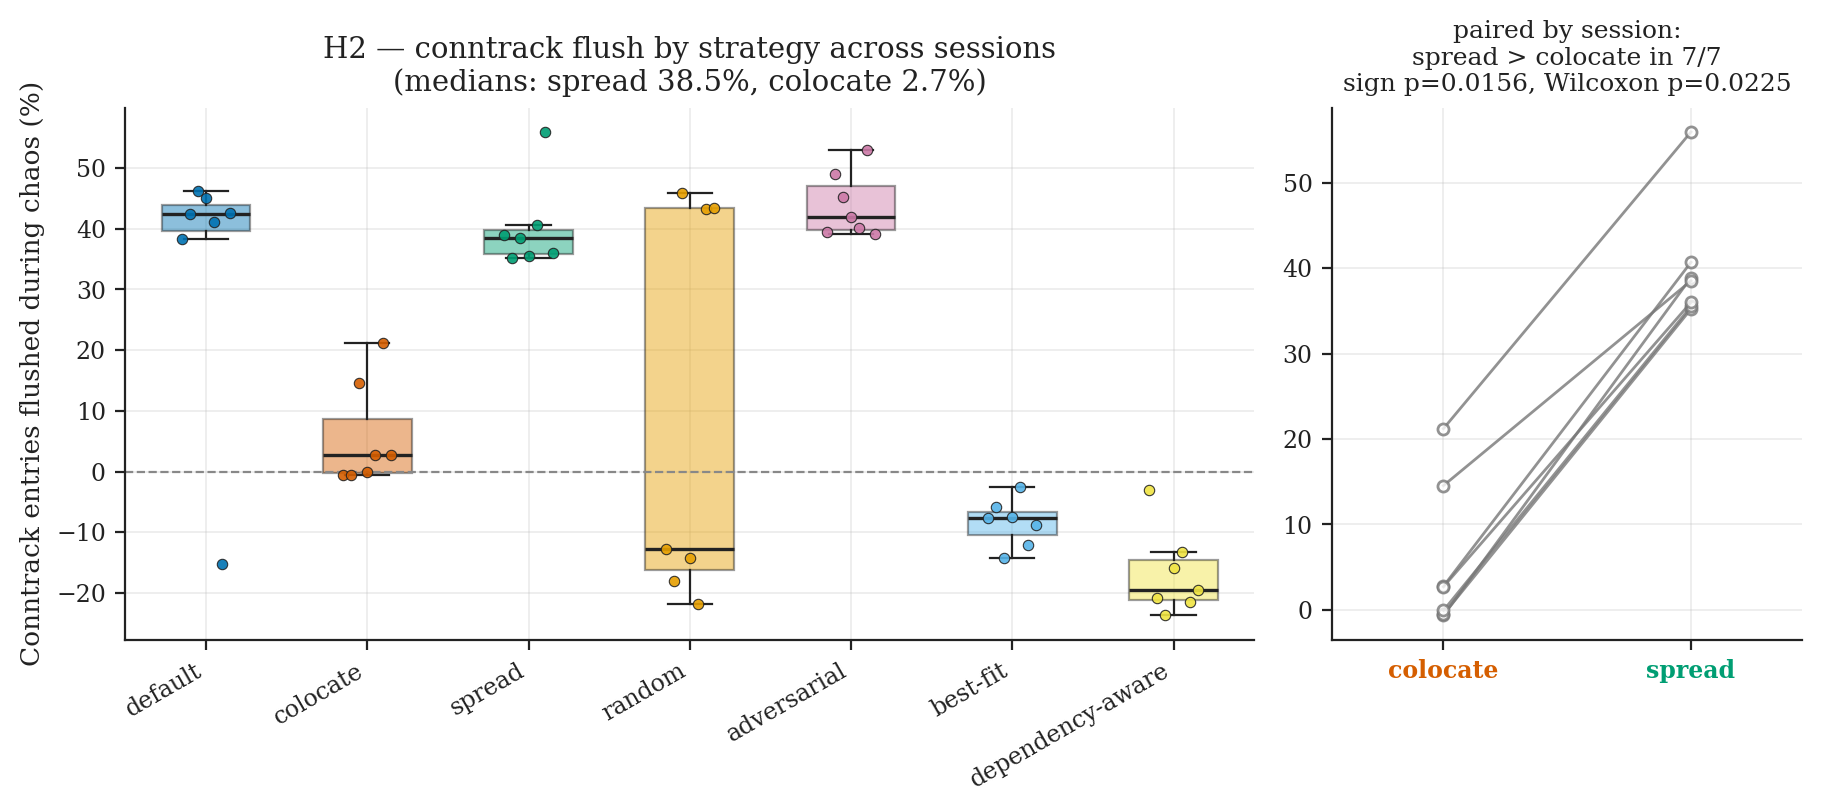
\includegraphics[width=\textwidth]{fig-05-h2-conntrack.png}
  \caption{Conntrack flush \% per strategy across the seven sessions
    (spread > colocate in all seven; note \texttt{default} flushes as hard as \texttt{spread}
    ($\sim$42\%) while \texttt{dependency-aware}/\texttt{best-fit} show \emph{negative} flush --- entries
    grow during chaos --- consistent with the flush tracking placement-dependent
    state composition rather than a fixed per-strategy quantity).}
  \label{fig:h2-conntrack}
\end{figure}

\section{H3 --- The mechanism is decoupled from the user-visible outcome}\label{sec:h3}

\textbf{Statement.} The reproducible mechanism (H2) does not translate into a
reproducible user-visible outcome on the fault-dependent routes beyond a
run-level confound.

\textbf{Result --- decoupling supported (campaign + three pilot tests).} Across the
7 sessions (49 strategy-cells): conntrack flush $\rightarrow$ \textbf{dependent}-route p95 is
\textbf{$\rho = 0.07$ ($p = 0.65$)} and \textbf{decoupled by TOST}, while the \textbf{control}
route shows $\rho = 0.29$ ($p = 0.043$) --- the mechanism correlates with the route
that does \emph{not} depend on the killed service: the signature of a run-level
confound, not propagation. The only dependent-significant association
(TCP-retransmit delta, $\rho = -0.32$) is \emph{negative} --- opposite a propagation
story. Pilot agreement: pooled $\rho = 0.15$ n.s.; the one significant mechanism
(CoreDNS p99) stronger on control (0.54) than dependent (0.31); within-run
mean $\rho \approx +0.10$; robust to route reclassification.

No statistics needed for the headline table: \texttt{dependency-aware} has the
\emph{worst} mechanism (conntrack +20\%) and the \emph{best} dependent-route error rate
(1.4\%); \texttt{spread} flushes 9$\times$ more than \texttt{colocate} yet they tie on user-visible
error (8.0\% vs 8.9\%).

Why would a kernel-layer signature this reproducible fail to reach the user
routes? The plausible mechanism reading: under single-replica churn the
user-visible outcome is dominated by the outage itself --- the target's only
replica is gone for the same deletion-to-ready cycle whatever the topology ---
while client retries and timeouts mask the differences in reconvergence
timing that the conntrack signature represents. This interpretation is ours
(per the convention of Chapter~\ref{ch:discussion}); what is measured is the layer split, and
\S\ref{sec:decoupling} develops the account in full.

\begin{figure}[tb]
  \centering
  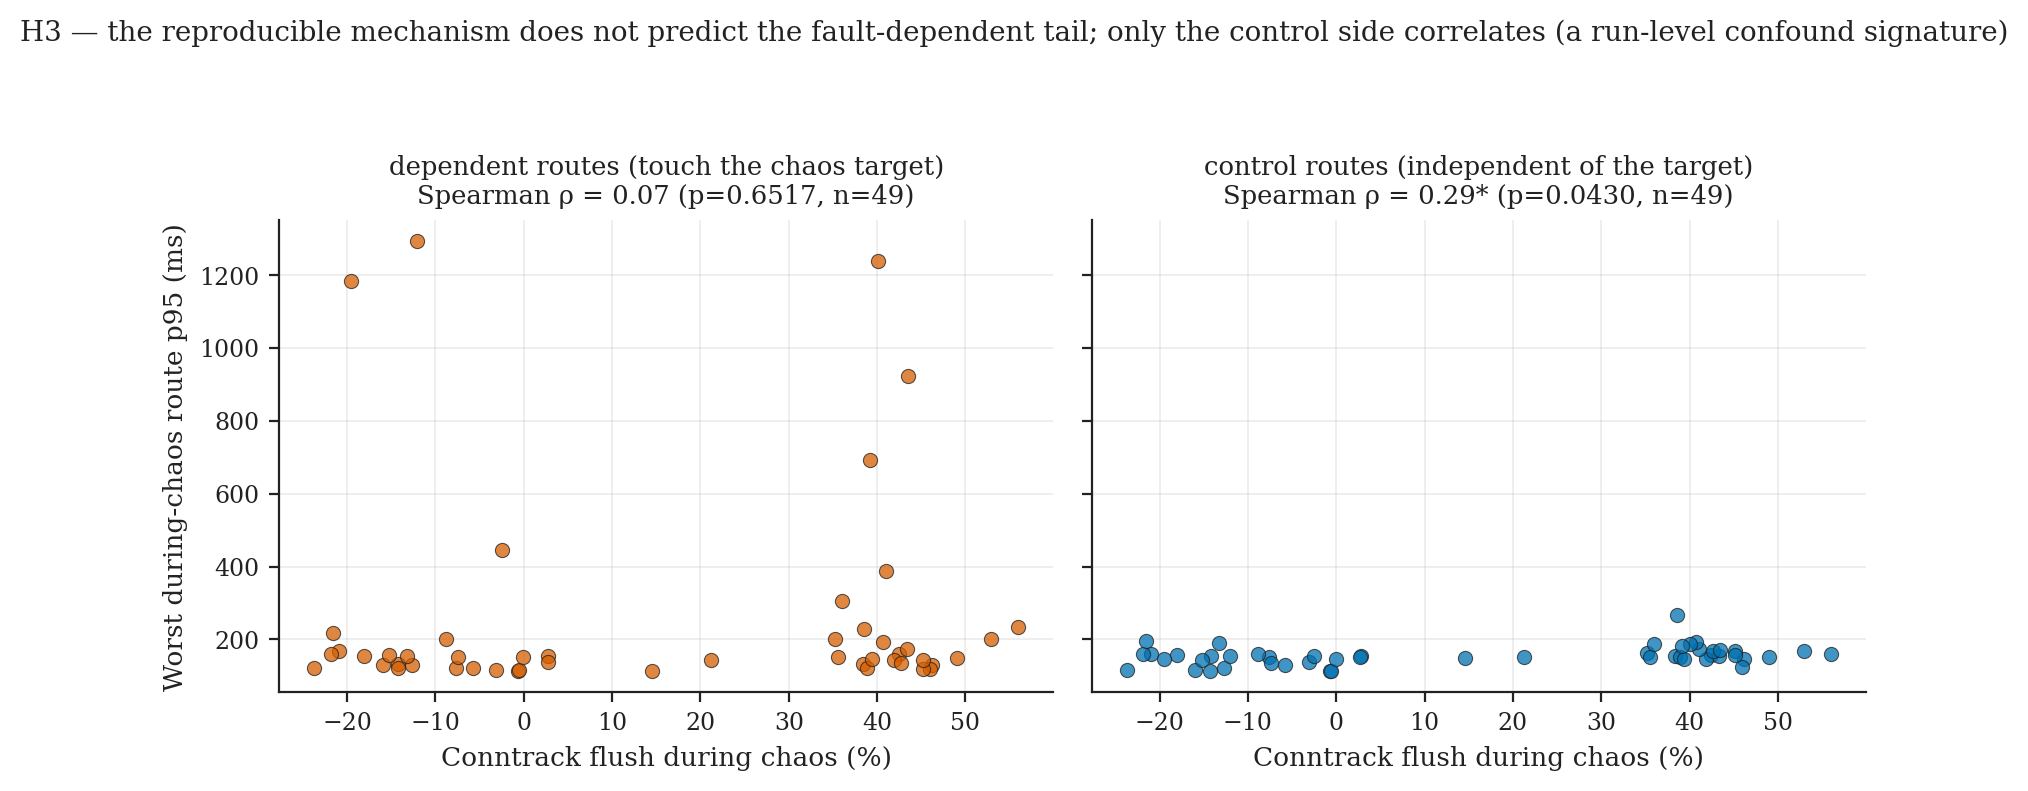
\includegraphics[width=\textwidth]{fig-06-h3-scatter.png}
  \caption{Mechanism-vs-outcome scatter (dependent vs control routes
    per strategy-cell): the flush correlates with the route that does \emph{not}
    depend on the killed service.}
  \label{fig:h3-scatter}
\end{figure}

\section{H4 --- Under load contention, placement moves the mechanism, not (reproducibly) the user}\label{sec:h4}

This section contains the first of two results the provenance discipline
retracted --- the demonstration that the gate works as designed (\S\ref{sec:campaign}).

\textbf{Result --- mechanism replicates; user layer does not.} Two $i = 4$ batches
(the second with fully clean, doctor-gated provenance):

\begin{itemize}
\item \emph{Replicated}: east-west inter-service p95, median spread/colocate ratio
  \textbf{1.39$\times$ (batch A)} and \textbf{1.36$\times$ (batch B)} --- co-location keeps calls
  node-local.
\item \emph{Not replicated}: user-facing during-load ratios collapsed from $\sim$2.1--2.4$\times$
  (batch A, dependent > control) to $\sim$1.05--1.40$\times$ (batch B, dependent $\approx$
  control --- no dependency specificity). The dirty pilot's ``co-location $\sim$3$\times$
  better at the user layer'' reading did not survive replication.
\end{itemize}

\textbf{No user-visible placement effect is claimed under load.} The finding
matches the churn result: layered decoupling holds across both fault classes.

Why does the east-west effect replicate while the user routes do not? The
inter-service hop is the direct mechanical path placement changes --- a call
either crosses a node boundary or it does not --- whereas a user-facing route
aggregates many hops and, under a 200-user spike, sits behind cluster-wide
queueing noise that affects every route alike. The locality term plausibly
drowns in that first-order saturation before it reaches the front end. This
interpretation is ours (per the convention of Chapter~\ref{ch:discussion}); \S\ref{sec:tradeoff} prices the
east-west locality face that does replicate against its availability
counterpart.

\section{H5 --- A graph-derived metric separates node-local from spreading placements}\label{sec:h5}

This section contains the second result the provenance discipline retracted:
replication kept the separation but took back the headline correlation (\S\ref{sec:campaign}).

\textbf{Result --- the two-regime separation replicates across two independent
batches; a continuous law does not.} Across all 8 strategies under a
200-user spike ($i = 4$ per batch):

\begin{center}
\begin{tabular}{lrrrr}
\toprule
\textbf{strategy} & \textbf{frac (batch 1)} & \textbf{EW p95 (batch 1)} & \textbf{frac (batch 2)} & \textbf{EW p95 (batch 2)} \\
\midrule
\textbf{colocate} & 0.00 & \textbf{33.9} & 0.00 & \textbf{33.2} \\
\textbf{best-fit} & 0.13 & \textbf{35.3} & 0.00 & \textbf{35.7} \\
dependency-aware & 0.73 & 42.6 & 0.73 & 43.8 \\
spread & 0.73 & 43.5 & 0.73 & 44.2 \\
baseline & 0.70 & 43.5 & 0.78 & 41.7 \\
adversarial & 0.80 & 43.5 & 0.80 & 42.0 \\
default & 0.78 & 45.5 & 0.82 & 41.6 \\
random & 0.80 & 43.9 & 0.80 & 42.8 \\
\bottomrule
\end{tabular}
\end{center}

In \textbf{both} batches the two node-local placements (cross-node fraction $\approx$ 0)
occupy the two lowest east-west tails of eight --- per-batch null probability
$1/28 \approx 0.036$, jointly $\approx 0.0013$ --- at $\sim$\textbf{1.25$\times$} below the spreading cluster
($\sim$34.6 vs $\sim$43.5 ms medians in batch 1; $\sim$34.5 vs $\sim$42.4 ms in batch 2). The
fraction, computed pre-chaos from the dependency graph + actual
\texttt{podPlacements}, captures that separation.

The \emph{continuous} correlation did \textbf{not} replicate: batch 1's Spearman
$\rho = 0.79$ ($n = 8$, carried by \texttt{best-fit}'s intermediate 0.13 point) collapsed
to \textbf{$\rho = 0.25$ (n.s.)} in batch 2, where \texttt{best-fit} packed fully (fraction
0.00) and the spreading cluster showed no internal trend. We therefore claim
H5 as a \textbf{replicated two-regime separator}, not a smooth predictor --- and
quote $\rho = 0.79$ only alongside $\rho = 0.25$.

Secondary findings: locality is \textbf{not unique to \texttt{colocate}} (\texttt{best-fit}'s
bin-packing lands node-local in both batches --- any node-packing placement
gets the benefit); \textbf{\texttt{dependency-aware} did not deliver} (fraction 0.73 in
both batches --- the BFS partition did not co-locate communicating services as
intended; its tail $\approx$ spread's both times).

Caveats: the user layer stays weak ($\sim$1.3$\times$, not dependency-specific); batch
2's launching tree was dirty in non-code files only (deck binary + figure
PNGs; running code = \texttt{e543fbb}); the aggregate score is \textbf{saturated} in
these load runs (batch 1: all eight strategies scored 100; CIs overlap in
both batches --- H1 again, and the saturation \S\ref{sec:decoupling} discusses); this is
\textbf{validation of a static separator}, not of the locality concept (\S\ref{sec:positioning}).

\begin{figure}[tb]
  \centering
  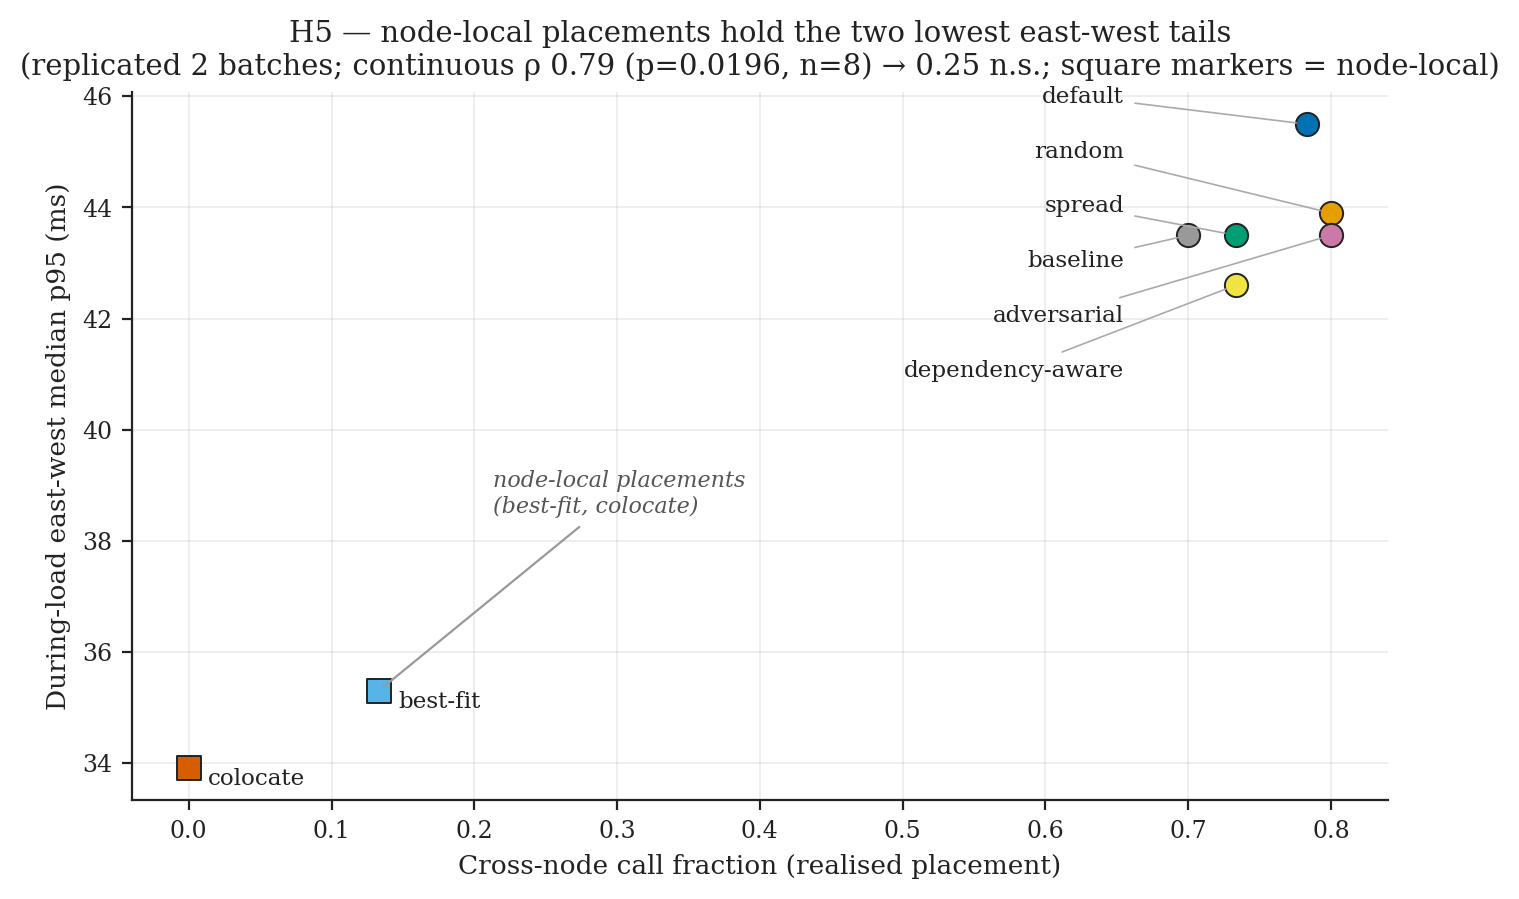
\includegraphics[width=\textwidth]{fig-07-h5-fraction-vs-tail.png}
  \caption{Cross-node fraction vs during-load east-west p95 (batch 1;
    square markers = the node-local pair). Batch 2 reproduces the separation with
    \texttt{best-fit} at fraction 0.00; see the table above.}
  \label{fig:h5-fraction}
\end{figure}

\section{H6 --- Co-location is a latency/availability trade-off}\label{sec:h6}

\textbf{Result --- supported and reproduced (two doctor-clean node-drain batches:
$i = 1$ and $i = 3$).} Draining the node hosting \texttt{productcatalogservice}:

\begin{center}
\begin{tabular}{llll}
\toprule
\textbf{placement} & \textbf{services on drained node} & \textbf{blast radius (observed)} & \textbf{target recovery (mean)} \\
\midrule
\textbf{colocate} & 11 / 11 & \textbf{11 --- whole app offline} & \textbf{$\approx$ 10.3 s} \\
\textbf{spread} & 2 / 11 & \textbf{2 (18\%)} & \textbf{$\approx$ 2.6 s} \\
\bottomrule
\end{tabular}
\end{center}

Observed blast equals placement-predicted blast in every iteration, measured
from EndpointSlice outage troughs (15 s sampling) --- not the score, which is
unusable here (a drain leaves every Litmus probe \texttt{Unknown}; H1 again).

\textbf{Gradient extension (6 placing strategies $\times$ $i = 3$, doctor-clean).}
The full gradient run confirms the relationship is exact across the
intermediate placements: \textbf{observed blast equals the placement-predicted
blast for every strategy} ---

\begin{center}
\begin{tabular}{llll}
\toprule
\textbf{strategy} & \textbf{services on drained node} & \textbf{blast (observed)} & \textbf{recovery (mean)} \\
\midrule
colocate & 11 & \textbf{11} & 10.8 s \\
random & 4 & \textbf{4} & 4.6 s \\
dependency-aware & 3 & \textbf{3} & 33.3 s \\
best-fit & 3 & \textbf{3} & 9.7 s \\
spread & 2 & \textbf{2} & 2.6 s \\
adversarial & 2 & \textbf{2} & 33.1 s \\
\bottomrule
\end{tabular}
\end{center}

Spearman(predicted, observed) = \textbf{1.0} ($n = 6$): per-node concentration
predicts the availability consequence exactly, the availability analogue of
H5's separator. \textbf{Recovery time, however, is \emph{not} monotone in blast} ---
intermediate-blast placements produced both the fastest (4.6 s) and slowest
(33.3 s) recoveries --- so the recovery claim is scoped to the
colocate-vs-spread extremes contrast (10.3 s vs 2.6 s, $\sim$4$\times$), where it
reproduced across both original batches. (Recovery times are not pooled
across batches: the gradient run is a distinct batch and reads colocate at
10.8 s vs 10.3 s in the two-point batches.)

\textbf{The trade-off is the finding}: the same co-location that gives the lowest
east-west tail (H5: $\sim$33--34 ms in both batches) gives a 100\% single-drain
outage; \texttt{spread} is the mirror. One graph property, two opposing measured
consequences. Framing per scope-of-claims: this is the \textbf{quantification of a
known qualitative trade-off}, not its discovery (the full novelty framing
lives in \S\ref{sec:tradeoff}) --- the empirical content is that it materializes under real
chaos with no partial survival, holds across the full strategy gradient, and
drives a measured recovery penalty at the extremes.

Caveats: single-replica, single cluster; recovery non-monotonicity above.

\begin{figure}[tb]
  \centering
  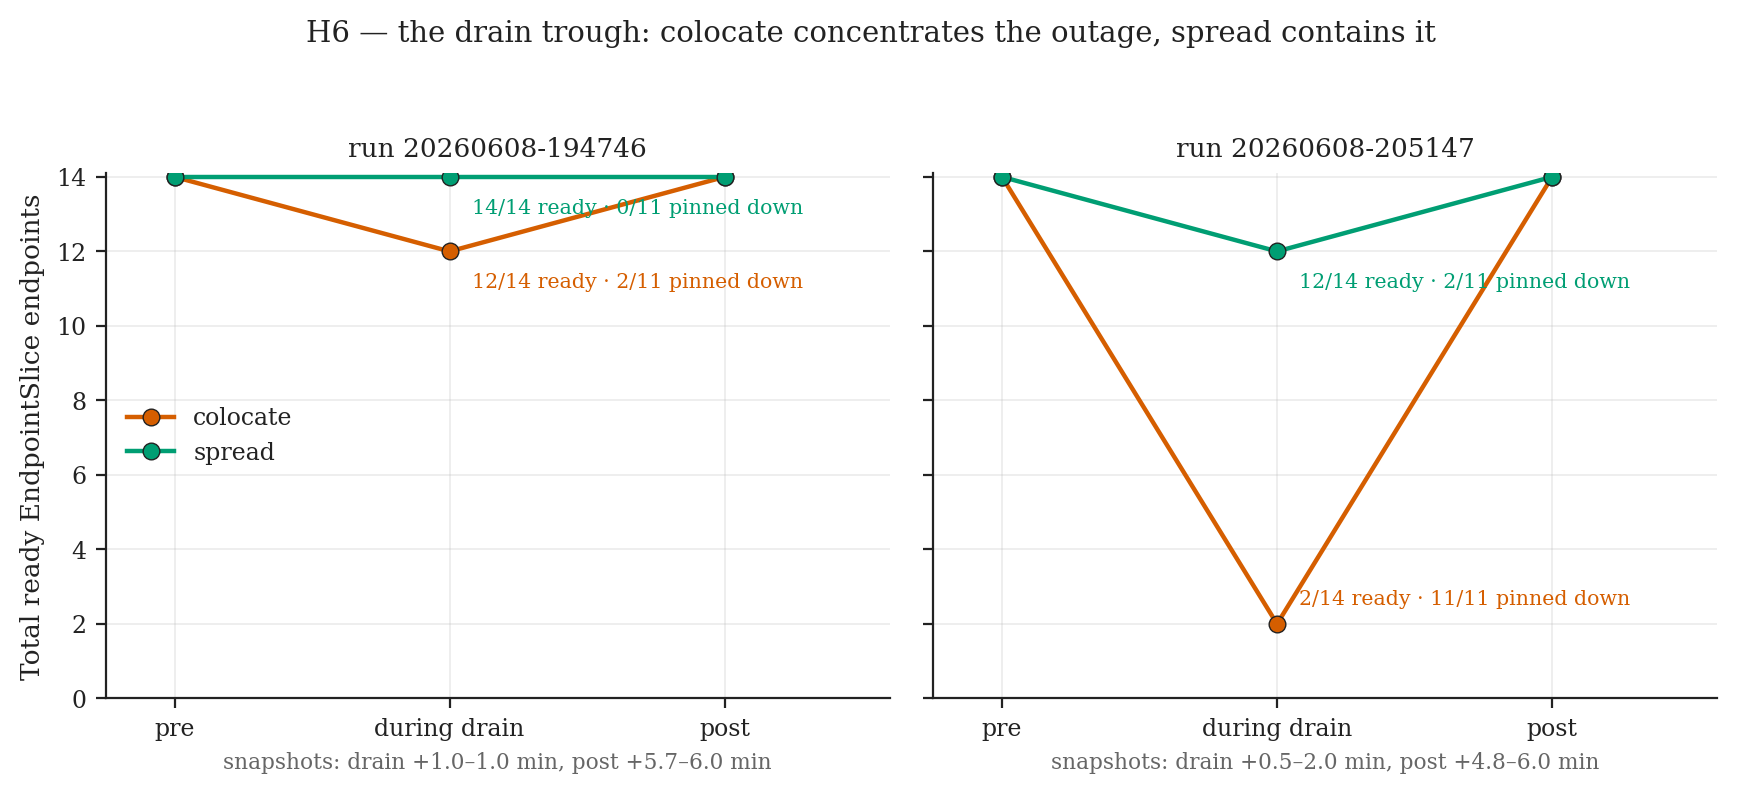
\includegraphics[width=\textwidth]{fig-08-h6-trough-timeline.png}
  \caption{EndpointSlice ready-count trajectory through the drain
    (colocate vs spread; the $i = 3$ batch catches the trough that a fixed-offset
    snapshot missed --- the motivation for the 15 s trough sampler).}
  \label{fig:h6-trough}
\end{figure}

\begin{figure}[tb]
  \centering
  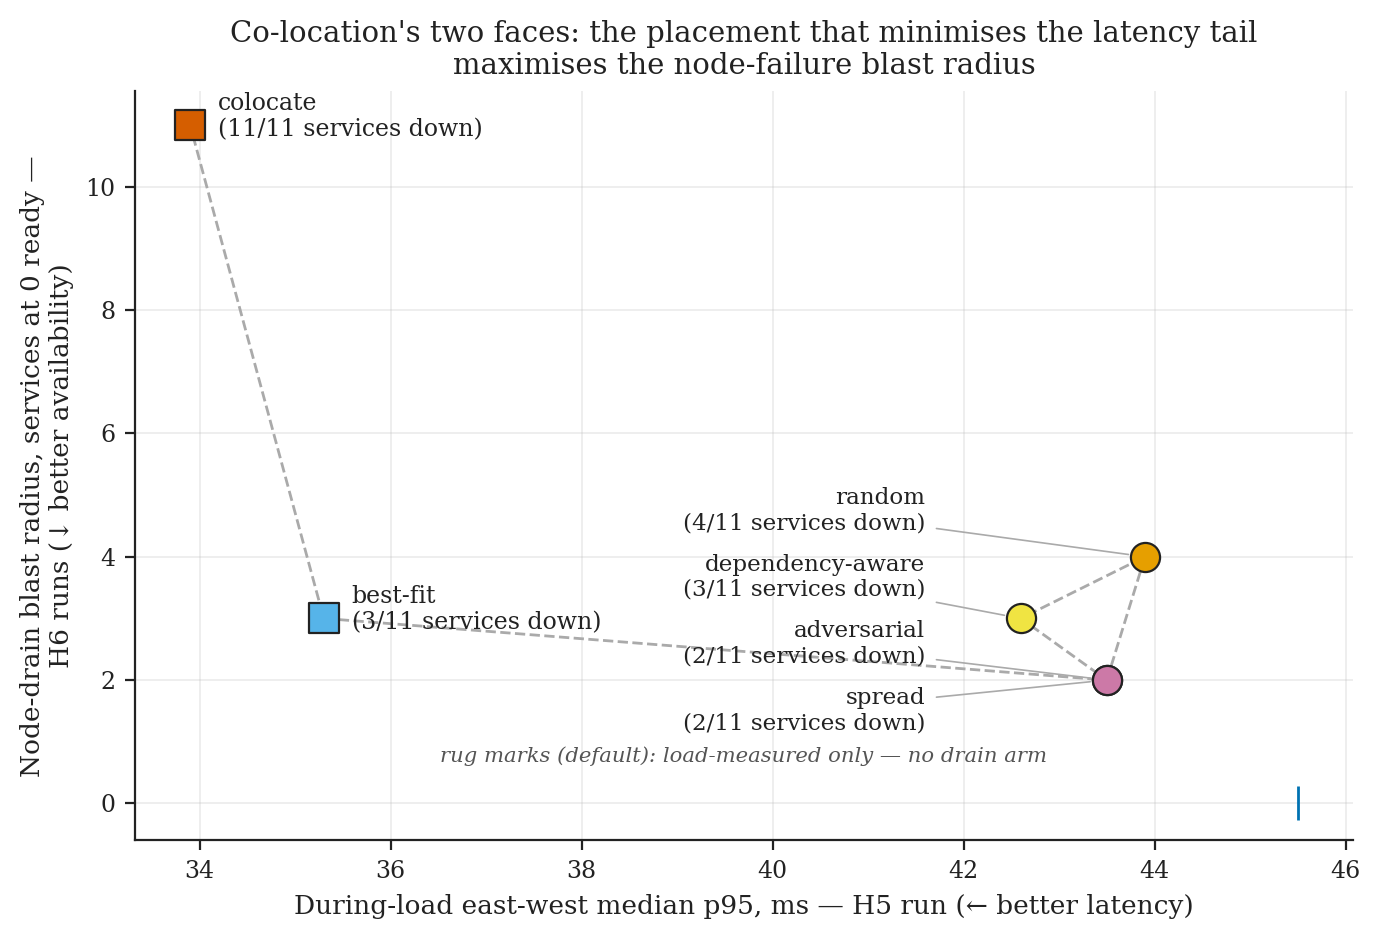
\includegraphics[width=\textwidth]{fig-09-tradeoff.png}
  \caption{The headline figure: the same placements plotted on the
    east-west latency axis (H5) and the node-drain blast-radius axis (H6),
    opposing gradients of co-location.}
  \label{fig:tradeoff}
\end{figure}

\section{Per-claim evidence table}\label{sec:evidence-table}

\begin{center}
\footnotesize
\begin{tabular}{p{0.24\textwidth}p{0.15\textwidth}p{0.21\textwidth}p{0.07\textwidth}p{0.21\textwidth}}
\toprule
\textbf{Claim} & \textbf{Data} & \textbf{Test} & \textbf{Figure} & \textbf{Archived run(s) (Appendix~\ref{app:provenance})} \\
\midrule
H1: score cannot rank under session variance & s01--s07, 147 iterations & variance partition; ICC + cluster-bootstrap CI; power/MDE & \ref{fig:h1-dist}, \ref{fig:h1-icc} & run-20260608-233543 \ldots{} run-20260610-130249 (7 archives) \\
\addlinespace
H2: conntrack flush, spread > colocate & s01--s07 & sign test (7/7, $p = 0.0156$); Wilcoxon ($W = 0$, $p = 0.0225$) & \ref{fig:h2-conntrack} & same 7 archives \\
\addlinespace
H3: mechanism $\perp$ dependent-route outcome & s01--s07, 49 cells & Spearman dep 0.07 vs ctrl 0.29*; TOST equivalence & \ref{fig:h3-scatter} & same 7 archives \\
\addlinespace
H4: east-west replicates, user layer does not & 2 $\times$ $i = 4$ load batches & ratio replication (1.36--1.39$\times$); dep-vs-ctrl collapse & --- & run-20260607-193053, run-20260607-221822 \\
\addlinespace
H2 mechanism: UDP-pool decomposition & 2 $\times$ $i = 1$ probe runs + 5 s protocol samples & composition: UDP $-$50--58\% vs TCP growth under spread & --- & run-20260610-200013, run-20260610-201131; \texttt{data/conntrack-probe/} \\
\addlinespace
H5: cross-node fraction separates node-local from spreading & 2 $\times$ (8 strategies $\times$ $i = 4$) & lowest-2-of-8 ranks in both batches (joint $\approx$ 0.0013); $\rho = 0.79 \rightarrow 0.25$ & \ref{fig:h5-fraction}, \ref{fig:tradeoff} & run-20260608-070638, run-20260610-202426 \\
\addlinespace
H6: blast radius + recovery trade-off & 2 node-drain batches + 6-strategy gradient & predicted = observed blast every iteration; gradient $\rho = 1.0$ ($n = 6$); recovery contrast at extremes & \ref{fig:h6-trough}, \ref{fig:tradeoff} & run-20260608-194827, run-20260608-205229, run-20260610-172430 \\
\bottomrule
\end{tabular}
\end{center}

\section{What the gate retracted}\label{sec:retractions}

Two of this study's most striking numbers appear nowhere among its claims,
and that is a result in itself. The dirty H4 pilot read as ``co-location $\sim$3$\times$
better at the user layer''; the clean, doctor-gated replication collapsed the
user-facing ratios to $\sim$1.05--1.40$\times$ with no dependency specificity, and the
reading was retracted (\S\ref{sec:h4}). H5's batch-1 continuous correlation (Spearman
$\rho = 0.79$) collapsed to $\rho = 0.25$ n.s.\ in batch 2, and only the two-regime
separation is claimed (\S\ref{sec:h5}). In both cases the provenance-and-replication
gate (\S\ref{sec:campaign}) did exactly what it was designed to do: it caught the most
quotable numbers in the study and removed them. A method that retracts its
own most striking results is the credibility argument for contribution 3 ---
the campaign protocol's discipline is demonstrated here, not merely stated
(\S\ref{sec:not-claimed}, \S\ref{sec:conclusion}).

% Ported from thesis/06-discussion.md — wording unchanged.
\chapter{Discussion}\label{ch:discussion}

\section{Layered decoupling holds across both fault classes}\label{sec:decoupling}

Under churn, placement leaves a large, reproducible footprint at the kernel
layer (H2) that never reaches the user (H3), while the aggregate score is too
noisy to see anything at all (H1). Load contention --- the regime where the
user-visible outcome \emph{is} latency --- was expected to differ, and does not: the
east-west mechanism reproduces (1.36--1.39$\times$) but the user-layer effect
collapsed in the clean replication (H4). Placement moves the mechanism in
both regimes; the user layer follows in neither.

Once \texttt{pod-delete} is understood as a \emph{churn} fault, this is the expected
shape rather than a surprise. The injected event is the disappearance and
recreation of a service's only replica. During the kill window the service
is simply gone: every dependent request fails identically whether the
surviving services are packed on one node or spread across four, because
what governs the user-visible outcome is availability dynamics --- the
deletion-to-ready cycle of the single replica --- and not the topology around
it. What placement \emph{does} govern is how much networking state the churn
event invalidates: a spread placement holds the target's connections across
node boundaries, so the kill cycle tears down and reconverges a large
fraction of per-node conntrack state (H2's 38.5\% median flush), where a
co-located placement holds them node-locally and barely registers (2.7\%).
The mechanism layer is exactly where a topology variable should leave its
mark under a churn fault --- and the user layer is exactly where it should
not, because the user-facing damage is dominated by the outage itself.
This interpretation is ours; what is measured is the layer split (H2, H3),
and the single-replica scoping of it is stated in \S\ref{sec:generalizes}.

Load contention is the regime where the same logic was expected to break:
the application stays fully available, the outcome under stress is latency,
and latency is what locality moves. The mechanism half of that expectation
holds --- co-location keeps east-west calls node-local and reproducibly
lowers the inter-service tail in both batches (H4) --- but the effect
attenuates before it reaches the user-facing routes, whose during-load
ratios collapsed to $\approx$1.1--1.4$\times$ with no dependency specificity in the clean
batch. In this environment the user-facing tail under a 200-user spike is
dominated by the cluster-wide saturation itself --- every route, dependent or
not, is queueing --- so the placement-attributable east-west difference is a
second-order term. We mark this as interpretation: what replication
establishes is only that the mechanism effect survives and the user-layer
effect does not (\S\ref{sec:h4}).

It is worth being precise about \emph{how} the aggregate score fails, because it
fails differently in each regime --- and the failure modes compound rather
than cancel. Under churn the score is \textbf{noisy}: it varies, but 96.7\% of
its variance is run-to-run and iteration noise, so the between-strategy
signal is undetectable at any feasible iteration count (H1). Under load it
is \textbf{saturated}: all eight strategies scored 100 in the H5 run, because
the application stays available under contention and availability is what
the probes measure --- the score has no dynamic range exactly where the
latency action is (\S\ref{sec:h5}). Under node drain it is \textbf{absent}: the drain
takes down the infrastructure the Litmus probes themselves depend on,
every probe returns \texttt{Unknown}, and the score is undefined just when the
availability outcome is most dramatic (\S\ref{sec:h6}). A single-number instrument
would need to be unreliable in none of these ways to rank placements
across fault classes; this one is unreliable in all three, each for a
different, diagnosable reason. That is the constructive content of H1: not
that scoring is hopeless, but that the failure modes are layer- and
regime-specific, and an evaluation pipeline must know which one it is in.

The decoupling result also returns something to the work it is positioned
against. MicroRes's premise (\S\ref{sec:positioning}) is that resilience consists in
degradation \emph{failing to disseminate} from system metrics to user metrics ---
their index scores that dissemination. H3 and H4 are, in effect, a
mechanism-level account of when and why that dissemination fails under a
manipulated variable: under churn the system-layer perturbation
(conntrack reconvergence) is real, large, and placement-controlled, yet
dissemination to the user layer is statistically absent; under load the
east-west perturbation likewise stops short of the user-facing routes.
Where MicroRes treats non-dissemination as the \emph{definition} of resilience
to be scored, this thesis measures it as a \emph{phenomenon} with a fault-class
structure --- they score the decoupling, we measure its mechanism --- and the
two readings are complementary rather than competing.

The negative findings of Appendix~\ref{app:negative} belong in this picture, because they
explain why the \emph{obvious} experimental designs would have probed the wrong
layer entirely. The catalog contention faults --- CPU and memory hogs --- are
absorbed by the very resource-isolation machinery (CFS quota, requests,
kubelet eviction ordering) that they try to stress: the hog spends its own
budget, or evicts itself first, and the application never becomes
resource-bound (\S\ref{sec:fault-classes}, Appendix~\ref{app:negative}). A study that ran ``placement $\times$ cpu-hog''
and found nothing would have learned a property of the fault, not of
placement. Recognizing the hogs as layer-mismatched instruments --- and
replacing them with genuine load --- is what made the H4/H5 regime testable
at all, and we present that redirect as a methodological contribution in
its own right.

\section{The trade-off as the operator takeaway}\label{sec:tradeoff}

H5 and H6 are the same graph property read on two axes: co-location minimizes
the east-west tail ($\sim$33--34 ms vs $\sim$42--44 ms across both batches) and maximizes node-failure blast
radius (11/11 vs 2/11) and recovery ($\approx$10.3 s vs $\approx$2.6 s). The cross-node
fraction prices the \emph{latency} face before any chaos; the services-per-node
concentration prices the \emph{availability} face. An operator does not get to
optimize one without paying the other --- and neither face is visible in the
aggregate score.

Figure~\ref{fig:tradeoff} renders this as a single picture: per-strategy cross-node
fraction on one axis, with the east-west p95 (H5) and the node-drain blast
radius (H6) as opposing gradients. Reading it left to right, the node-local
placements (\texttt{colocate}, \texttt{best-fit}) sit at the latency optimum and the
availability pessimum; the spreading placements sit at the mirror point.
The figure is the thesis's headline because both gradients are \emph{measured on
the same placements}, in the same environment, from the same dependency
graph --- the latency face under a 200-user load (run-20260608-070638), the
availability face under node drains across two clean batches. The pair
H5+H6 is what elevates the study's mostly-decoupling story into actionable
structure: the placement decision is not ``does placement matter?'' but
``which face of this measured trade-off does your SLO price higher?''

We are explicit about what is and is not new here. That concentrating
workload into one failure domain enlarges the blast radius when that domain
fails is a known qualitative principle --- it is the premise of cell-based
architecture guidance in industry
(\citealp{aws-cellbased};
its cell-placement guidance treats co-locating partition keys as a
qualitative factor, and its only blast-radius quantification is 1/N scoping
arithmetic), the motivation for Kubernetes' own topology-spread constraints
(\citealp{kep895},
which asserts high availability qualitatively and quantifies only
scheduler-internal criteria), and the resilience rationale in Medea
(\citealp{garefalakis2018medea}
--- qualitative motivation plus a trace-driven unavailability analysis,
performed separately from its performance evaluation, with no injected-fault
or blast-radius experiment). The H6 prediction taken alone is also
near-definitional (drain a node, lose the pods on it). The contribution is
the \emph{quantification on the placement axis with both faces measured on the
same workload under identical placements} --- which none of those sources do: the same placements that H5
prices for latency are drained and priced for availability, the predicted
blast radius materializes exactly in every iteration, and concentration
additionally drives a $\sim$4$\times$ recovery-time penalty that is not definitional
(it arises from rescheduling contention when 11 evicted pods restart at
once). H6 as it stands is a two-point contrast between the extremes; the
intermediate-concentration gradient is the natural completion (\S\ref{sec:h6}, \S\ref{sec:future-work}).

\section{The H2 mechanism: attribution with protocol scoping}\label{sec:h2-mechanism}

The conntrack-flush signature maps onto the reconvergence window the
Kubernetes SIG-Scalability network-programming SLO defines, but the
attribution must be protocol-scoped: upstream maintainers document
kube-proxy's \emph{active} conntrack flush on endpoint churn as \textbf{UDP-only}
(kubernetes/kubernetes \#48370, \#108523, \#126130; TCP entries are deliberately
never actively flushed --- \#100698, \#104098). Online Boutique's east-west
traffic is gRPC/\textbf{TCP}, which initially made the attribution look
problematic: how can a UDP-only cleanup path produce a large flush in a
TCP workload? A dedicated protocol-composition probe answered this
empirically (per-node \texttt{conntrack -L} protocol counts sampled every 5 s
through one full kill cycle under each placement; raw data in
\texttt{thesis/data/conntrack-probe/}, archived runs \texttt{run-20260610-200013} and
\texttt{run-20260610-201131}).

The probe's window-robust findings keep \textbf{both} candidate mechanisms in
play and locate the placement-dependence precisely. First, \textbf{TCP dominates
the conntrack table under both placements ($\approx$80 \%+ of entries) and drops
sharply at the kill cycles in both} (spread $-$28 \%, colocate $-$21 \% within
one cycle): kube-proxy has no TCP conntrack-deletion path --- a verified
property of every existing call site from the exec-based cleaner ($\le$ v1.31,
\texttt{conntrack -D \ldots{} -p udp}) through the netlink reconciler ($\ge$ v1.32, which
filters \texttt{protocol != UDP}; SCTP was treated like UDP pre-reconciler), though
not an API guarantee --- so these drops are kernel-side teardown of flows
traversing the killed pod. Precisely: connection close transitions entries
into short-timeout conntrack states (\texttt{nf\_conntrack\_tcp\_timeout\_close} = 10 s,
\texttt{\_close\_wait} = 60 s, \texttt{\_fin\_wait} and \texttt{\_time\_wait} = 120 s, vs five days for
\texttt{ESTABLISHED}), so FIN/RST-driven teardown expires entries within $\le$ 120 s of
the kill --- consistent with the observed within-cycle drops --- while abruptly
severed connections whose peers never emit a sequence-valid close can linger
in \texttt{ESTABLISHED}, which is why the drop is partial rather than total. None
of this needs kube-proxy involvement. Second, \textbf{the clearly placement-dependent
component is UDP (DNS)}: under steady load \texttt{spread} sustains $\sim$4$\times$ more UDP
entries than \texttt{colocate} (chaos-window medians 910 vs 224) --- spreading the
dependency graph across nodes means inter-service calls cross the network,
connection churn drives DNS re-resolution, and those UDP flows are exactly
the traffic class kube-proxy's documented UDP-only cleanup acts on.
\texttt{colocate}'s UDP count even \emph{rises} during chaos (restart-driven lookups),
underlining that the UDP level tracks churn topology, not a fixed quota.

What the probe deliberately does \textbf{not} establish is the apportionment:
with one iteration per placement and a pre-chaos window contaminated by the
load generator's start-up ramp (UDP transiently spiked to 5,485 inside
spread's baseline), pre-vs-during percentages from the probe are not
meaningful, and the campaign's 38.5 \% vs 2.7 \% flush medians cannot be
split between the TCP-teardown and UDP-cleanup paths from this data. The
defensible attribution is therefore: the H2 signature is real, reproducible,
and placement-dependent; both kernel TCP teardown and the UDP/DNS pool
visibly participate; the UDP pool is the component whose \emph{size} placement
controls; and the exact shares await a steady-state, multi-iteration probe
(\S\ref{sec:future-work}). The probe is quoted for composition and event timing only; the
campaign's seven sessions carry the statistical weight. Conntrack behaviour
also changed materially across K8s v1.31--v1.32; the result is pinned to
v1.28.6 (\S\ref{sec:environment}).

\section{L1--L3: inapplicable in this regime, not refuted}\label{sec:l1l3}

The literature-derived predictions --- L1 \emph{colocate is worst} (Bubble-Up,
Quasar), L2 \emph{spread isolates best} (Medea), L3 \emph{recovery time predicts
resilience} (Tail at Scale) --- are best described as \textbf{inapplicable in the
single-replica churn regime tested}, not refuted: churn is not the
contention regime they were written for; recovery's two-phase split is
unstable run-to-run, so L3 has no stable relationship to find on either side.
Under load --- their actual regime --- the locality intuition holds at the
mechanism layer but no user-layer ordering is asserted (H4).

Earlier drafts of this work stated these results as refutations --- ``the
spread-is-safer intuition is disproven'' --- and the correction is itself one
of the study's findings about how placement advice should be handled. The
contention literature's predictions come with an implicit regime attached:
Bubble-Up and Quasar model steady-state interference between co-located
workloads, and Medea's spread prescription protects multi-replica services
against failure-domain loss. Single-replica \texttt{pod-delete} churn satisfies
neither premise --- there is no sustained contention, and there is no second
replica for isolation to save --- so finding the predictions inert there is
evidence about their \emph{scope}, not their truth. The study's own data makes
the same point from the other side: in the regimes the predictions were
written for, they resurface with the expected sign --- under load contention
the locality logic behind L1/L2 holds at the mechanism layer (H4, H5), and
under node failure the isolation logic behind L2 is precisely what H6
measures, with spread limiting blast radius exactly as Medea's reasoning
implies. The practical lesson is that placement advice is \emph{fault-class
advice}: a recommendation like ``spread for resilience'' is meaningful only
together with the fault class and replication regime it was derived in, and
transplanting it across regimes --- as a single aggregate score implicitly
invites --- is how operators end up optimizing against the wrong failure
mode.

\section{Practical implications}\label{sec:implications}

\begin{itemize}
\item \textbf{Don't rank placements by one score.} In this regime the aggregate score
  cannot rank strategies at any feasible iteration count (H1); a score-based
  ``winner'' is noise.
\item \textbf{Measure the layer your fault class perturbs.} Churn shows up in
  endpoint/conntrack reconvergence; load in east-west tails; node failure in
  EndpointSlice availability troughs. A single user-layer or score-layer
  probe misses all three.
\item \textbf{Price co-location's two faces.} Co-location is simultaneously the best
  latency placement and the worst node-failure placement here (H5 + H6);
  choose per workload SLO, not per folklore.
\item \textbf{The cross-node fraction prices the latency face pre-chaos.} It is
  computable from the dependency graph + a proposed placement before any
  experiment --- a cheap static screen (with H6's concentration count as its
  availability counterpart).
\end{itemize}

Each of these is an implication of a measured result, and each inherits that
result's scope. The first follows from H1's variance decomposition --- and
from the three regime-specific score failure modes diagnosed in \S\ref{sec:decoupling} --- and
it is the one with the sharpest operational edge: an evaluation pipeline
that runs a handful of chaos iterations per placement and picks the
highest-scoring one is, in this regime, selecting on noise. The second is the constructive alternative the
three-layer design demonstrates: each fault class deposited its placement
signal in a different, \emph{predictable} layer, so instrumenting that layer
(conntrack/EndpointSlice for churn, east-west route tails under load,
ready-endpoint troughs under drain) recovers the signal the score loses.
The third and fourth turn H5+H6 into a screening procedure: given a
dependency graph and a candidate placement, the cross-node fraction prices
the latency face and the services-per-node concentration prices the
availability face, both before any experiment is run --- with chaos
experiments then reserved for validating the shortlisted candidates rather
than searching the whole space.

These are statements about this regime and this environment, with the
portability boundary stated in \S\ref{sec:generalizes}'s table. What is portable is the
\emph{method}: manipulate placement, measure at the
layer the fault class perturbs, control the user layer with
dependent-vs-control routes, gate every number on provenance, and audit the
aggregate score's reliability before trusting it to rank anything.

% Ported from thesis/07-threats.md — wording unchanged.
\chapter{Threats to validity \& scope}\label{ch:threats}

% Ported from hypotheses.md "Scope & threats" + scope-of-claims.md.
% Keep the two tables in sync with those sources.

This chapter states the boundary of every claim. We organize the threats in
the standard vocabulary. \textbf{Construct validity} asks whether the measured
quantities mean what the claims need them to mean: whether the probe-based
aggregate score measures ``resilience'' at all is itself under test (H1
quantifies its reliability rather than assuming it), the conntrack flush
percentage is a \emph{proxy} for reconvergence whose causal decomposition is
explicitly pending (\S\ref{sec:h2-mechanism}), and the \texttt{metricAvailability} bookkeeping exists
because a missing metric silently read as zero would corrupt the construct
it stands for. \textbf{Internal validity} asks whether observed differences are
attributable to the manipulated variable: the threats here are run-level
drift, placement mismatch, and dirty provenance, and the defenses --- the
dependent-vs-control route split, within-run correlation,
\texttt{placementMatchRates}, and the \texttt{doctor --strict} gate --- are built into the
design (\S\ref{sec:three-layer}, \S\ref{sec:campaign}) rather than applied post hoc. \textbf{External validity} asks
how far the results carry: a single small virtualized cluster, one
workload, one Kubernetes version and kube-proxy mode, and a single-replica
deployment bound the claims tightly, which is why \S\ref{sec:generalizes} separates what
generalizes (the method, the mechanism's direction) from what does not (the
absolute values, anything multi-replica). \textbf{Conclusion validity} asks
whether the statistics support the inferences drawn: with 7 sessions and
$n = 3$ iterations per cell, the campaign leans on nonparametric tests,
cluster-bootstrap intervals, equivalence testing for the decoupling claims,
and explicit power/MDE calculations rather than significance hunting
(\S\ref{sec:statistics}). The tables below give the threat-by-threat detail.

\section{Threats and defences}\label{sec:threats-table}

\begin{center}
\footnotesize
\begin{tabular}{p{0.2\textwidth}p{0.32\textwidth}p{0.38\textwidth}}
\toprule
\textbf{Threat} & \textbf{Why it matters} & \textbf{Defence} \\
\midrule
\textbf{Single-replica design} & 100\% \texttt{pod-delete} guarantees the only instance disappears, which can swamp topology effects. & Scope the claim to \emph{single-replica churn} and layered measurement; multi-replica anti-affinity is named as future work, not claimed. \\
\addlinespace
\textbf{Small virtualized cluster} & Four 4 GiB KVM/QEMU workers may not generalize. & Claim bounded external validity; report \emph{direction} and \emph{mechanism}, not absolute latency values. \\
\addlinespace
\textbf{Version sensitivity} & kube-proxy / conntrack behaviour evolves across releases (materially in v1.31--v1.32). & Archive exact Kubernetes (v1.28.6), CNI, runtime, kube-proxy mode/conntrack settings, ChaosProbe commit (\texttt{runMetadata} / manifests); present as a measurement study of a specific environment. \\
\addlinespace
\textbf{Placement mismatch} & The scheduler may not realize the intended placement. & Report \texttt{placementMatchRates}; flag or exclude mismatched iterations. \\
\addlinespace
\textbf{Run-to-run drift} & Iteration noise can dominate (H1: 37.6\% run-to-run + 59.1\% iteration variance). & Independent single-commit sessions as unit of analysis; strategy order fixed; pre/post snapshots; run modelled as a random/blocking effect; cluster-bootstrap CIs. \\
\addlinespace
\textbf{Dirty provenance} & Untracked files / missing metadata undermine credibility (the H4 pilot lesson). & Never quote results from runs failing \texttt{doctor --strict}; the dirty H4 pilot was replaced by two doctor-gated $i = 4$ batches. \\
\addlinespace
\textbf{Metric-availability gaps} & Missing PromQL queries can manufacture fake zeros. & \texttt{metricAvailability} distinguishes ``not collected'' from ``collected zero'' (e.g.\ kube-proxy programming latency is recorded as \emph{uncollected} here, and anchors the mechanism only conceptually). \\
\addlinespace
\textbf{Overclaiming causality} & Run-level slowness can confound correlations. & Dependent-vs-control routes + within-run correlation; TOST for equivalence claims; causal language reserved for the manipulated variable (placement). \\
\bottomrule
\end{tabular}
\end{center}

Two of these threats deserve a sentence beyond the table. The
single-replica design is not only a threat but a \emph{scoping instrument}: it
is what makes \texttt{pod-delete} a pure churn fault (the outage is total by
construction, so any placement signal must appear at a non-availability
layer), and it is simultaneously what excludes the multi-replica
anti-affinity regime from every claim. And the run-to-run drift row is not
an admission that the environment was too noisy --- quantifying that noise
and what it does to score-based ranking \emph{is} H1; the campaign design exists
because the drift was measured, not despite it.

\section{What generalizes vs.\ what does not}\label{sec:generalizes}

\begin{center}
\footnotesize
\begin{tabular}{p{0.32\textwidth}p{0.18\textwidth}p{0.4\textwidth}}
\toprule
\textbf{Aspect} & \textbf{Generalizes?} & \textbf{Why / caveat} \\
\midrule
The \emph{method} (placement-aware, cross-layer, provenance-gated chaos evaluation) & \textbf{Yes} & The framework and analysis discipline are reusable on any cluster/workload. \\
\addlinespace
The \emph{direction} of the H2 mechanism effect (spread flushes more conntrack than colocate under churn) & \textbf{Direction only} & Reproducible here; absolute values are environment-specific. \\
\addlinespace
Absolute metric values (latency, recovery s, flush \%) & \textbf{No} & Tied to a small virtualized 5-node cluster. \\
\addlinespace
Mechanism behaviour (conntrack, kube-proxy sync) & \textbf{Environment-contingent} & Depends on CNI, kube-proxy mode (ipvs here), kernel/conntrack settings --- archived per run so the scope is explicit. \\
\addlinespace
The score-instability finding & \textbf{This regime} & Established for single-replica \texttt{pod-delete}; ``cannot rank placement strategies under session variance'', not ``scores don't work''; not asserted for multi-replica or contention-dominated regimes. \\
\addlinespace
The H5 separator & \textbf{As a validated static screen here} & Two-regime separation replicated across two independent batches ($\rho$ 0.79 $\rightarrow$ 0.25: the continuous correlation did not replicate and is not claimed); validation of the metric, not of the locality concept. \\
\addlinespace
The H6 trade-off & \textbf{Qualitatively known; quantified here} & Two-point contrast, single-replica; the \emph{quantification} is this environment's. \\
\addlinespace
Anything about multi-replica / HA failover & \textbf{Not in scope} & Structurally excluded by the single-replica design (\S\ref{sec:future-work}). \\
\bottomrule
\end{tabular}
\end{center}

The asymmetry of this table is deliberate. The portable row is the first
one: the measurement design, the campaign protocol, and the analysis
scripts transfer to any cluster and workload unchanged, and a replication
on different infrastructure is the most valuable follow-up this study
could receive. Everything below it degrades gracefully from ``direction
only'' to ``not in scope'' --- and where a row says environment-contingent, the
archived manifests make the contingency checkable rather than vague: a
reader who wants to know whether a result could apply to their cluster can
compare their kube-proxy mode, conntrack settings, and Kubernetes version
against the archived fingerprint instead of guessing.

\section{Explicitly not claimed}\label{sec:not-claimed}

Per \texttt{scope-of-claims.md}:
no universal ``best'' placement strategy; no ``spread is worse/disproven''; no
proven causality for the conntrack mechanism (mechanistic consistency, not
controlled causal proof); no generalization to Kubernetes clusters broadly;
no ``the score identifies the best strategy''; no unqualified ``reproducible''
(only the mechanism metrics reproduce, and only with the archived rerun
package).

These exclusions are commitments, not disclaimers: each one names a stronger
claim that the data could be mistaken to support and that we decline. The
list was not assembled at writing time; it accumulated during the study, as
earlier, stronger phrasings (``refuted'', ``spread is disproven'', a $\sim$3$\times$ user-layer
advantage) failed replication or scrutiny and were retired (\S\ref{sec:h4},
\S\ref{sec:l1l3}). Where this document's prose and that scope statement could ever be
read to disagree, the scope statement governs.

\chapter{Conclusion \& future work}\label{ch:conclusion}

\section{Conclusion}\label{sec:conclusion}

This thesis asked: \textbf{under which chaos fault classes does pod placement
measurably affect mechanism-level behaviour and user-visible outcomes in a
Kubernetes microservice application, and when do aggregate resilience scores
obscure those effects?} Answered through a pre-registered, Holm-corrected
confirmatory family, the result is a real mechanism whose reach is rigorously
bounded.

The positive thread is the \emph{mechanism}. Placement reproducibly moves a
UDP-conntrack reconvergence signature, and that effect is significant in every
campaign: it is placement-dependent under churn (H2), it interacts with
replication under node-drain (H3's error face, where anti-affine replication
fully rescues the user-route error rate), and it is the one scorecard layer with
near-perfect test-retest reliability (H5, mechanism ICC 0.994 vs a naive
aggregate's 0.066). A NodeLocal DNSCache intervention removes the conntrack drop
under both placements --- the one actionable lever the study confirmed.

The bound is what pre-registration makes precise. No confirmatory hypothesis
clears its registered bar (\S\ref{sec:family-holm}): the dose-response is
detectable but below the 15\,\% SESOI (H1); placement-dependence replicates with
the \emph{opposite} sign, packing concentrating more per-node conntrack churn
than spreading, so the conjunction fails (H2); replication's rescue is clear on
the error face but the trough-depth co-primary could not adjudicate it on this
placement (H3); and the scorecard's availability layer is unreliable under churn
(H5). The latency$\leftrightarrow$availability frontier is likewise
degenerate on the availability face under pod-delete (H4) --- both reflecting
that pod-delete produces no sustained availability outage to discriminate on. Placement moves the
mechanism; at the pre-registered bar, it does not move the user-visible
placement, availability, and dose-response outcomes the hypotheses predicted.

The three contributions of \S\ref{sec:contributions} carry this answer within the
boundary of Chapter~\ref{ch:threats}. The empirical finding --- a real,
DNS-mediated, placement-dependent conntrack mechanism whose user-visible reach is
bounded --- is a statement about a single-replica baseline on one small
virtualized v1.28.6/ipvs cluster (\S\ref{sec:generalizes}), never ``spread is
worse'' or a best strategy. ChaosProbe and the deposit-before-analysis campaign
protocol are the portable parts: any cluster and workload can rerun this design,
and every number traces to an archived, hash-stamped run
(Appendix~\ref{app:provenance}).

The methodological point is the one we would have the field retain. Chaos
evaluation of placement needs \textbf{layered measurement, pre-registration, and
provenance-gated replication, not a single score}: each fault class deposited
its placement signal in a specific layer, a one-number instrument's availability
component was unreliable or undefined exactly where it mattered, and freezing the
hypotheses and effect-size bars before collection is what turned ``we observed
placement effects'' into the more honest ``here is exactly which effects survive
a strict bar, and which do not.''

\section{Future work}\label{sec:future-work}

\subsection*{Second-workload external validity (the highest-value next step)}

The single largest threat (\S\ref{sec:generalizes}) is that all results come from
one workload. The natural next step is to replicate the confirmatory family on a
second microservice application (e.g.\ a Consul/gRPC workload such as
DeathStarBench hotelReservation). A scoping attempt surfaced a concrete blocker
worth recording: that workload's inter-service gRPC clients enter a keepalive
reconnection storm (server-side \texttt{too\_many\_pings} GoAway responses) after
the per-iteration clean-baseline restart, leaving the search path unavailable
for many minutes and false-tainting every iteration's readiness gate, even
though the latency data collected once it recovers is clean. The
restart-for-clean-baseline protocol is thus incompatible with workloads prone to
such storms without one of: a much longer readiness budget, a per-workload skip
of the per-iteration restart (a documented protocol deviation), or tuning the
workload's gRPC keepalive (a change to the system under test). Resolving that
choice is the prerequisite for clean second-workload data.

\subsection*{Decomposing and extending the mechanism}

\begin{itemize}
\item \textbf{Conntrack-drop apportionment.} The drop has both a kernel TCP
  teardown component and the placement-dependent UDP/DNS pool the cache removes
  (\S\ref{sec:h2-mechanism}); a steady-state, multi-iteration protocol-composition
  probe would apportion the two, converting the study's most reproducible signal
  from mechanism-consistent to causally decomposed.
\item \textbf{A rescue-margin the depth face can express.} H3's trough-depth
  co-primary could not adjudicate rescue because the registered absolute one-pod
  margin coincided with the $r{=}1$ dynamic range on this placement; a margin
  defined relative to the realized $r{=}1$ depth (or an integrated outage =
  depth\,$\times$\,duration metric) would let a future pre-registration test the
  depth face on its merits.
\item \textbf{Denser dose levels and other faults.} Finer cross-node-fraction
  steps around the detected (sub-SESOI) trend, and a fault that varies the
  availability face while retaining a latency face, would let the frontier (H4)
  realize the trade-off it is degenerate on here.
\end{itemize}

\subsection*{Environment and scope}

Larger and bare-metal clusters, other CNIs and kube-proxy modes (iptables,
nftables --- the de-scoped direction-transfer comparison), multi-replica
workloads beyond the node-drain regime H3 reaches, production traffic, and
integrating the cross-node fraction into a scheduler as a scoring plugin. The
common thread is the method: each of these runs on the same layered,
pre-registered, provenance-gated protocol this thesis contributes, and each
would sharpen --- not merely extend --- the boundary of where placement matters.


% ------------------------------ Appendix --------------------------------
\appendix
% Ported from thesis/09-appendix-provenance.md — wording unchanged.
% The markdown file holds both appendices; here they become Appendix A and B.

\chapter{Run provenance}\label{app:provenance}

Generated from the per-archive \texttt{artifact-manifest.json} files in
\texttt{chaosprobe/dist/} (schema 2.0.0). Shared environment
fingerprint across \textbf{all} archives: Kubernetes \textbf{v1.28.6}, kube-proxy mode
\textbf{ipvs} (conntrack \texttt{maxPerCore} 32768, \texttt{min} 131072, TCP established 24 h /
close-wait 1 h), containerd 1.7.11, Ubuntu 22.04.3 LTS, Calico CNI, namespace
\texttt{online-boutique}, git \texttt{dirty: false}, \texttt{provenanceWarnings: []}.

\begin{quote}
Naming note: a run's \texttt{results/<timestamp>/} directory is stamped at launch,
its \texttt{runId} at archive time --- they can differ by seconds-to-minutes (e.g.\
\texttt{results/20260607-193021} $\leftrightarrow$ \texttt{run-20260607-193053}). The runId is canonical.
\end{quote}

\begin{center}
\scriptsize
\setlength{\tabcolsep}{3pt}
\begin{tabular}{p{0.145\textwidth}p{0.07\textwidth}p{0.09\textwidth}p{0.165\textwidth}p{0.25\textwidth}p{0.015\textwidth}p{0.16\textwidth}}
\toprule
\textbf{runId} & \textbf{batch} & \textbf{commit} & \textbf{archive} & \textbf{strategies $\times$ fault} & \textbf{i} & \textbf{role} \\
\midrule
run-20260607-123106 & 2026-06-07 & \texttt{50773a2c6f57} & \texttt{run-20260607-123106.tar.gz} & baseline, colocate, default, spread $\times$ \{pod-delete, node-memory-hog\} & 4 & node-memory-hog negative finding (Appendix~\ref{app:negative}) \\
\addlinespace
run-20260607-193053 & 2026-06-07 & \texttt{41e2c9a3e8bd} & \texttt{run-20260607-193053.tar.gz} & baseline, colocate, default, spread $\times$ load-contention & 4 & H4 batch A \\
\addlinespace
run-20260607-221822 & 2026-06-07 & \texttt{829a52adb693} & \texttt{run-20260607-221822.tar.gz} & baseline, colocate, default, spread $\times$ load-contention & 4 & H4 batch B (clean replication, 0 taints) \\
\addlinespace
run-20260608-070638 & 2026-06-08 & \texttt{a881a12344be} & \texttt{run-20260608-070638.tar.gz} & all 8 $\times$ load-contention & 4 & H5 (cross-node fraction) \\
\addlinespace
run-20260608-233543 & 2026-06-08 & \texttt{68151857f9a4} & \texttt{run-20260608-233543.tar.gz} & all 8 $\times$ pod-delete & 3 & campaign \textbf{s01} \\
\addlinespace
run-20260609-072731 & 2026-06-09 & \texttt{c8511f2fa093} & \texttt{run-20260609-072731.tar.gz} & all 8 $\times$ pod-delete & 3 & campaign \textbf{s02} \\
\addlinespace
run-20260609-154457 & 2026-06-09 & \texttt{c8511f2fa093} & \texttt{run-20260609-154457.tar.gz} & all 8 $\times$ pod-delete & 3 & campaign \textbf{s03} \\
\addlinespace
run-20260609-194339 & 2026-06-09 & \texttt{a80d25b5cb6f} & \texttt{run-20260609-194339.tar.gz} & all 8 $\times$ pod-delete & 3 & campaign \textbf{s04} \\
\addlinespace
run-20260610-050703 & 2026-06-10 & \texttt{a80d25b5cb6f} & \texttt{run-20260610-050703.tar.gz} & all 8 $\times$ pod-delete & 3 & campaign \textbf{s05} \\
\addlinespace
run-20260610-090416 & 2026-06-10 & \texttt{a80d25b5cb6f} & \texttt{run-20260610-090416.tar.gz} & all 8 $\times$ pod-delete & 3 & campaign \textbf{s06} \\
\addlinespace
run-20260610-130249 & 2026-06-10 & \texttt{a80d25b5cb6f} & \texttt{run-20260610-130249.tar.gz} & all 8 $\times$ pod-delete & 3 & campaign \textbf{s07} \\
\addlinespace
run-20260608-194827 & 2026-06-08 & \texttt{97799efa5ea5} & \texttt{run-20260608-194827.tar.gz} & colocate, default, spread $\times$ node-drain & 1 & H6 two-point batch ($i = 1$) \\
\addlinespace
run-20260608-205229 & 2026-06-08 & \texttt{3d437cdd2e4a} & \texttt{run-20260608-205229.tar.gz} & colocate, default, spread $\times$ node-drain & 3 & H6 two-point batch ($i = 3$) \\
\addlinespace
run-20260610-172430 & 2026-06-10 & \texttt{6696e6be175d} & \texttt{run-20260610-172430.tar.gz} & 6 placing strategies $\times$ node-drain & 3 & H6 gradient (doctor-clean) \\
\addlinespace
run-20260610-200013 & 2026-06-10 & \texttt{e543fbb9e5fe} & \texttt{run-20260610-200013.tar.gz} & spread $\times$ pod-delete & 1 & H2 protocol probe (spread) \\
\addlinespace
run-20260610-201131 & 2026-06-10 & \texttt{e543fbb9e5fe} & \texttt{run-20260610-201131.tar.gz} & colocate $\times$ pod-delete & 1 & H2 protocol probe (colocate) \\
\addlinespace
run-20260610-202426 & 2026-06-10 & \texttt{e543fbb9e5fe} & \texttt{run-20260610-202426.tar.gz} & all 8 $\times$ load-contention & 4 & H5 \textbf{batch 2} (doctor-strict 0 errors; launching tree dirty in non-code files only: deck binary + 3 figure PNGs) \\
\bottomrule
\end{tabular}
\end{center}

``All 8'' = baseline, default, colocate, spread, adversarial, random, best-fit,
dependency-aware. ``Independent single-commit session'' means each session ran
on one commit throughout; sessions may share a commit (s02/s03; s04--s07) ---
independence is per \emph{invocation/day}, not per commit.

Each archive carries the SHA-256 of the exact scenario YAML injected (e.g.\
s07 \texttt{pod-delete.yaml} = \texttt{d1a57729\ldots c79a58}) and of every data file
(\texttt{summary.json}, per-strategy JSON, charts).

\section{Claims $\rightarrow$ runs mapping}\label{sec:claims-runs}

\begin{center}
\footnotesize
\begin{tabular}{p{0.42\textwidth}p{0.5\textwidth}}
\toprule
\textbf{Claim} & \textbf{Archived run(s)} \\
\midrule
\textbf{H1, H2, H3} (7-session churn campaign, 147 iterations) & s01--s07 = run-20260608-233543, run-20260609-072731, run-20260609-154457, run-20260609-194339, run-20260610-050703, run-20260610-090416, run-20260610-130249 \\
\addlinespace
\textbf{H4} (load contention, two batches) & run-20260607-193053 (A) + run-20260607-221822 (B, clean) \\
\addlinespace
\textbf{H5} (cross-node fraction, 8 strategies, two batches) & run-20260608-070638 (batch 1) + run-20260610-202426 (batch 2) \\
\addlinespace
\textbf{H6} (node-drain blast radius, two batches) & run-20260608-194827 ($i = 1$) + run-20260608-205229 ($i = 3$) (run dirs contain colocate/default/spread; H6 quotes the colocate-vs-spread contrast) \\
\addlinespace
\textbf{H6 gradient} (6 strategies $\times$ node-drain $\times$ $i = 3$) & run-20260610-172430 (\texttt{doctor --strict} clean; observed blast = predicted for all 6 strategies, Spearman $\rho = 1.0$) \\
\addlinespace
\textbf{H2 protocol-composition probe} (2 $\times$ $i = 1$ pod-delete, spread/colocate) & run-20260610-200013 (spread) + run-20260610-201131 (colocate); raw 5-s protocol samples in \texttt{thesis/data/conntrack-probe/} \\
\addlinespace
\textbf{H7} (discussion-tier, \S\ref{sec:future-work}) & derived from s01--s07 (analysis-only; \texttt{campaign\_status.py}) \\
\addlinespace
Pooled pilot (H1/H2/H3 corroboration only) & pre-campaign mixed-version \texttt{results/} runs --- \textbf{pilot tier, not archive-clean; never quote as findings} \\
\addlinespace
node-memory-hog / hog negative findings & run-20260607-123106 (+ 1-iteration 100\% probe, unarchived diagnostic) \\
\bottomrule
\end{tabular}
\end{center}

\chapter{Negative findings}\label{app:negative}

These are deliberate, documented dead-ends --- kept because they constrain what
fault classes can test placement on this class of cluster.

\section{CPU hog faults are absorbed by CFS (scores $\approx$ 100)}\label{sec:cpu-hog}

\begin{itemize}
\item \texttt{pod-cpu-hog} is CFS-capped at the container's own 200m CPU limit: the
  stress consumes the victim's quota, the app stays up, resilience score
  $\approx$ 100, no user impact. Its CPU-throttling side-signal is corroborating
  only (\S\ref{sec:h2}).
\item \texttt{node-cpu-hog} loads the node, but CPU \emph{requests} guarantee the light app
  pods their shares --- the app remains responsive; score $\approx$ 100.
\item Consequence: genuine contention must come from \textbf{load} (the 200-user
  Locust spike of H4/H5), not synthetic hogs.
\end{itemize}

\section{node-memory-hog self-eviction autopsy}\label{sec:memory-hog}

The $i = 4$ batch (run-20260607-123106) showed every node-memory-hog cell
scoring $\approx$ 100; a follow-up 1-iteration probe at
\texttt{MEMORY\_CONSUMPTION\_PERCENTAGE: 100} produced \textbf{zero} MemoryPressure, OOM,
or app-pod evictions (worker steady $\approx$ 75\% memory). Root cause, confirmed
against the \texttt{litmus-go} source: the percentage is computed against node
\textbf{capacity} and \textbf{clamped to allocatable} (not free memory), with no safety
margin --- on an already-utilized node the stressor cannot sustain its target,
and the \textbf{helper pod is the kubelet's first eviction victim}: it self-evicts
before any app pod is touched (per \texttt{litmus-go}'s
\href{https://github.com/litmuschaos/litmus-go/blob/master/chaoslib/litmus/node-memory-hog/lib/node-memory-hog.go}{\texttt{calculateMemoryConsumption}}:
percentage of node capacity, clamped to allocatable, no in-use accounting).
No percentage or
absolute-MiB setting fixes this on 4 GiB workers. Memory pressure becomes
placement-sensitive only via multi-replica + node-level exhaustion (\S\ref{sec:future-work},
option b path).

\section{H7 --- target-scoped cross-node fraction (suggestive only)}\label{sec:h7}

Recorded here for completeness: the global cross-node fraction does not
predict conntrack flush (single-session $\rho \approx 0.02$); scoping the fraction to
edges incident on the chaos target tracks it slightly better and firmed
mildly across the campaign ($\rho \approx 0.34$ target-scoped vs $\approx 0.30$ global at 7
sessions). Underpowered, wobbly across interim reads --- discussion-tier
material (\S\ref{sec:future-work}), not a claim.


% ---------------------------- Bibliography ------------------------------
% \nocite{*} prints the full annotated-bibliography source (references.md):
% entries referenced only by inline \href identifiers still appear.
\nocite{*}
\bibliography{references}

\end{document}
